\RequirePackage{fix-cm}

%% To Be Deleted... just a box to place for expected figures
\begin{filecontents*}{box.eps}
%!PS-Adobe-3.0 EPSF-3.0
%%BoundingBox: 19 19 221 221
%%CreationDate: Mon Sep 29 1997
%%Creator: programmed by hand
%%EndComments
gsave
newpath
  20 20 moveto
  20 220 lineto
  220 220 lineto
  220 20 lineto
closepath
2 setlinewidth
gsave
  .4 setgray fill
grestore
stroke
grestore
\end{filecontents*}

\documentclass[twocolumn,natbib,final]{svjour3}
\smartqed  % flush right qed marks, e.g. at end of proof

\usepackage{graphicx}
\graphicspath{ {./img/} {../img/} }
%\usepackage{hyperref}
% Tables
\usepackage{multirow}
\usepackage{colortbl}
\usepackage{booktabs}
\usepackage[algoruled,vlined]{algorithm2e}
\usepackage{amsmath,amsfonts,amssymb,amsxtra,amsbsy,amsopn}
\usepackage{paralist}
\usepackage{booktabs}
\usepackage{tabularx}
% argmax as math operator
\DeclareMathOperator*{\argmax}{arg\,max}

% todonotes, pass disable as option to also remove all notes
\usepackage[textsize=tiny]{todonotes}

% showlabels, useful for quickly ref command by viewing the pdf
% To remove pass final option
%\usepackage[inline]{showlabels}
%\renewcommand{\showlabelfont}{\scriptsize\scshape\bfseries\color{blue}}

\journalname{Autonomous Robots}
\begin{document}

%%%%%%%%%%%%%%%%%%%%%%%%%%%%%%%%%%%%%%%%%%%%%%%%%%%%%%%%%%%%%%%%%%%%%%%%%%%%%%%%
\title{%GPAtlasRRT: A probabilistic next-best tactile action strategy for object shape modeling and exploration
        GPAtlasRRT: A tactile exploration strategy for novel object shape modeling
  \thanks{This work is supported by EC-FP7-ICT-600918, PacMan.}
}
%\subtitle{GPAtlasRRT: Gaussian Process for shape modelling, continuation method on implicit manifolds (Atlas), rapidly-exploring random trees}
%\titlerunning{Short form of title}

\author{Carlos J. Rosales         \and
        Claudio Zito              \and
        Federico Spinelli         \and \\
        Marco Gabiccini           \and
        Jeremy L. Wyatt
}

\institute{C. J. Rosales, F. Spinelli, and M. Gabiccini \at
              Centro di Ricerca ``E. Piaggio'', Univ. di Pisa, Italy. \\
              %Tel.: +39 (050) 2217050\\
              \email{carlos.rosales@for.unipi.it}           %
           \and
           C. Zito and J. L. Wyatt \at
              Intelligent Robotics Laboratory, Univ. of Birmingham, UK.
              %Tel.: +44 (0) 121 415 8722\\
              %\email{cxz004@cs.bham.ac.uk}              %
}

\date{Received: date / Accepted: date}
% The correct dates will be entered by the editor


\maketitle

%%%%%%%%%%%%%%%%%%%%%%%%%%%%%%%%%%%%%%%%%%%%%%%%%%%%%%%%%%%%%%%%%%%%%%%%%%%%%%%%
\begin{abstract}
Information on object shape is a fundamental parameter for robot-object interaction to be successful. However, incomplete perception and noisy measurements impede obtaining accurate models of novel objects. Especially when vision and touch simultaneously are envisioned for learning object models, a representation able to incorporate prior shape knowledge and heterogeneous uncertain sensor feedback %flowing from different modalities 
is paramount to fusing them in a coherent way. Moreover, by embedding a notion of uncertainty in shape representation allows to more effectively bias the active search for new tactile cues. %to improve the model.
In this work, we use a Gaussian Process (GP) as such representation. Then, using the fact that the $0$-levelset of the GP --- the surface of the object --- is an implicitly defined manifold, we borrow the AtlasRRT algorithm concept to simultaneously: (i) build an atlas via continuation methods that locally parameterizes the object and that is used to select the next-best touch, and (ii) use an RRT-like strategy to devise directions for the expansion of the atlas to trade completeness in the exploration for efficiency. We integrate this strategy in a framework for iterative learning the object shape and implement a tactile exploration scenario in the bi-manual setting of our Vito robot. The experimental results confirm that the devised strategy yields better models compared to a naive strategy, and does it with a reduced number of touches. %% this depends on how we finally validate our strategy
\keywords{Next-best touch \and
          Shape modeling \and
          Tactile exploration}
\end{abstract}

%%%%%%%%%%%%%%%%%%%%%%%%%%%%%%%%%%%%%%%%%%%%%%%%%%%%%%%%%%%%%%%%%%%%%%%%%%%%%%%%
\section{Introduction}
\label{sec:intro}


General guidelines : \citet{Bajcsy1989Machine}

Active visual perception: \citet{Bajcsy1988Active}

Vision-based exploration is the most studied, perhaps due to its non-invasive nature, which avoids the contact between rigid bodies which is the cause of most headaches in physics modelling, simulation and control.

As very well said by \citet{Petrovskaya2011Global}, even when initial works date back to the 80's, tactile perception has not been addressed as deeply as the non-invasive counterpart, visual perception. Besides the need of being actively controlled, tactile sensors typically required ad-hoc mechanical devices.

``Touch-based perception has not been studied in as much depth
as vision because standardized touch sensors are not as easily
available. In many situations, tactile sensors have to be hand
crafted specifically for the robot and the task. This complicates
comparisons between methods and slows progress in tactile
perception. However, recently there has been a surge of interest
in the field due to the necessity of touch-based perception in
service applications''

Whereas \citet{Petrovskaya2011Global} is more interested in the object pose estimation problem, here we are more interested in the object shape modelling, sort of in the mapping of rather than localization in a SLAM problem.

On active touch sensing \citet{Prescott2011Active}

% There are two broad directions to represent object shapes. Use either an implicit or an explicit (a.k.a. parametric) representation. A good comparison between the two is provided by \citet{Pirri2006About}.

Regarding the shape representation...

Using Gaussian Process for shape modelling is having an intensive development in recent years \citep{Mahler2015Grasp,Rosales2014Active,Bjorkman2013Enhancing,Dragiev2011Gaussian}, due to its versatility to accomadate noisy information, provide smooth regression of data, and a natural way to fuse different sources of information \citep{Rasmussen2006Gaussian}.

Manifold gaussian process: \citet{Calandra2014Manifold} ``The quality of a Gaussian Process model strongly depends on an appropriate covariance function.''

The tree is constructed incrementally from samples drawn randomly from the search space and is inherently biased to grow towards large unsearched areas of the problem
Space-filling trees are 
Rapidly-exploring random trees \citet{LaValle2011Motion}

Continuation method for implicitly defined surfaces \citet{Henderson1993COMPUTING}

More general continuation method used in a more complex scenario combined with rapidly-exploring random trees \citep{LaValle2011Motion} by \citet{Jaillet2013Path}, where the idea is to explore the part of the manifold defined by several kinematic loop constraints that solves the motion planning query.

\citet{Zhu2009Nonrigid} succesfully recover non-rigid shape, means that gaussian processes can be used

\citet{Dragiev2011Gaussian} uses a squared-exponential-like covariance function. This is selection seems to be in agreement with the use is given to the shape estimation as a gradient field that drives the reach-to-grasp controller in a smooth way.

\citet{Rosales2014Active} exploits the Gaussian Process modelling the object shape to find geodesic trajectories on the surface that are later followed by an exploratory probe to gather frictional properties. However, no further use of that propery is given.

\citet{Mahler2015Grasp} proposes similar ideas as those given in \citet{Dragiev2011Gaussian}, in fact they follow the same covariance function for the shape modelling, but adds a local optimization step to have a more elaborated grasp controller that drives the hand to the most-likely succesful object grasp using a metric that involves the well-known Ferrari-Canny measure.

\citet{Williams2007Gaussian} derives the thin-plate covariance function for 3D shapes represented by implicit functions. The property of the thin-plate function to keep the tendency outside the training data is ideal for tactile exploration~\citep[Fig.~2]{Williams2007Gaussian}

The early work by \citet{Allen1987Robotic} presents a hierarchical representation of the object. The tactile exploration strategy to refine is driven by local geometry features. This is engaged by using surface tracing algorithms. In that work, it is literally said: ``Given a starting and ending point on a surface, the sensor traces along the surface reporting its contact positions and normals as it moves along.'' However, no indication is given in how to determine those starting and ending points on the surface.

\citet{Bjorkman2013Enhancing} follows the covariance function derived by \citet{Williams2007Gaussian}. This is the closest work to ours among the references. The main difference being the space in which the best-next exploratory action is computed and the terminal condition for the overal algorithm, and the descriptor. The Zernike moments imply an extra computation time, and lack of a probabilistic interpretation, which it is one of the good things about using Gaussian Process in first place. The exploratory actions are searched in a discrete space in the vertical direction and the approach angle, which seem extrinsic to the shape model. Using this space does not guarantee that the new observations will be on the desired shape region to be explored.  Finally, the number of actions, or touches in this case, are limited to a certain number, and then ordered according to the closes point on the implicit function with higher variance. In contrast, we set the highest expected variance in the shape prediction, so we explore until, probabilistically speaking, that goal is achieved.

These two works, \citet{Bjorkman2013Enhancing} and \cite{Dragiev2013Uncertainty} are very very similar to our approach.

% They claim that touch sensing is low bandwith, local, sequential process with better signal-to-noise ratio than vision. 

% Vision is global, has high bandwidth, and is noisy. Touch is a low bandwidth, local, sequential process with better noise properties than vision.

On how to do classification...

Shape representation and descriptor review \citet{Zhang2004Review}

In this work, we provide a systematic and coherent methodology to plan the next-best tactile exploratory action. The tactile exploratory action is intrinsically a contact hypothesis that need to be accepted or discarded after execution. Should the result be any of the two, it helps to improve the object shape prediction up to a pre-specified variability. In contrast to \citet{Bjorkman2013Enhancing}, we propose the same shape representation as descriptor for classification purposes using shape matching techniques~\citep{Belongie2002Shape}. The scope and problem statement is detailed in Sect.~\ref{sec:scope}. The proposed solution is broaden in Sect.~\ref{sec:solution}. The experimental results and discusion is presented in Sect.~\ref{sec:experiments}. Finally, the conclusions and points deserving further attention as given in Sect.~\ref{sec:conclusions}. 
%Reading the paper along watching the attached media is suggested for a better cath-up of the ideas.

%%%%%%%%%%%%%%%%%%%%%%%%%%%%%%%%%%%%%%%%%%%%%%%%%%%%%%%%%%%%%%%%%%%%%%%%%%%%%%%%
\section{Related work}
\label{sec:related}

%\subsection{State of the art}
%\label{sec:SoA}

One of the first attempts to exploit active tactile exploration with passive stereo vision for object recognition was proposed by Allen~\cite{Allen1987Robotic}. In that paper, a rigid tactile sensor traced along the object's surface in pre-defined movements. The work was later extended to develop different exploratory procedures to acquire and interpret 3D information on the surface shape \cite{Allen1990Acquisition}. The exploratory procedures were, however, selected by a human. Single-finger tactile exploration strategies for recognizing polyhedral objects have also been evaluated in simulation \cite{Roberts1990ICRA,Caselli1996ICRA}. 

Multiple fingers have also been used for tactile sensing. Moll and Erdmann~\cite{Moll2003STAR} presented a method for reconstructing the shape and motion of an unknown convex object using three sensorized fingers. In that approach, the object's friction properties must be known a priori and its surface must be smooth, lacking sharp edges and corners.

%The early work by \cite{Allen1987Robotic} presents a hierarchical representation of the object. The tactile exploration strategy to refine is driven by local geometry features. This is engaged by using surface tracing algorithms. In that work, it is literally said: ``Given a starting and ending point on a surface, the sensor traces along the surface reporting its contact positions and normals as it moves along.'' However, no indication is given in how to determine those starting and ending points on the surface. \cite{Allen1990Acquisition} blah blah

Tactile sensing has been used for localisation rather than surface recovery. Petrovskaya and Khatib \cite{Petrovskaya2011Global} used tactile exploration to localize an object of known shape. Since full Bayesian estimation of the pose of a free body is computationally expensive they approximated the posterior with particles. For a well-constrained object dataset the approach performs pose estimation in under one second with high reliability.

Bayesian methods have also been employed in shape estimation. Meier et al.\cite{Meier2011Probabilistic} performed tactile shape reconstruction using a Kalman filter. Efficient Bayesian inference using Gaussian processes has been used by various authors. For example, Sommer et al. \cite{Sommer2014Bimanual} proposed a method for bimanual compliant tactile exploration that used the GP representation to smooth the noisy point data, although they did not exploit the GP representation to derive the exploratory strategy.

Dragiev et al. \cite{Dragiev2011Gaussian} presented one of the first works to employ the Gaussian Process Implicit Surface (GPIS) representation for concurrent representation of the object shape and guidance of grasping actions. However, that paper utilized only the maximum a posteriori (MAP) estimate of the shape and thus did not utilise the ability of the Gaussian process to capture the uncertainty in the surface estimate. Later work, by the same authors, \cite{Dragiev2013Uncertainty} offered a way to prefer regions of the model with a particular certainty level in their shape estimate and introduced the notion of explore-grasp and exploit-grasp primitives.

Algorithms for selecting the sequence of touches have been developed by various authors. Bierbaum et al. \cite{Bierbaum2008Potential} guided tactile exploration using Dynamic Potential Fields for motion guidance of the fingers. They showed that grasp affordances can be generated from geometric features extracted from the contact points.

Bjorkman et al. \cite{Bjorkman2013Enhancing} showed how to build object models with a small number of tactile actions (each action involving multiple simultaneous touches by several tactile arrays) with the aim of categorisation, rather than shape recovery. They employed the GPIS representation mentioned above, with the kernal used by the GP being the thin plate covariance function derived by Williams \cite{Williams2007Gaussian}. A set of predefined tactile glances are performed on the object: however, these are not updated as the object model is refined. 

The main difference is that our approach is what we term {\em local tactile exploration} rather than {\em global tactile exploration}. By this we mean that our touch choices are constrained by the Atlas-RRT process to be considered first at points close to the already explored surface. The area considered for exploration grows outwards until a suitably uncertain point is found. This local exploration is very different from a global exploration strategy, in which any touch action can be considered. There is no inherent benefit to either approach, but local exploration allows us to define a series of touches across a contiguous area of hypothesized surface. Local exploration is a strategy often employed by humans. Both local and global strategies are important, but this is the first paper in which a local exploration strategy is combined with a GP representation of shape uncertainty. 

There are also other smaller differences: the space in which the next-best exploratory action is computed, the grain size to compute the predicted shape, and the terminating condition for the overall algorithm.
%//, and the descriptor used. 
Bjorkman et al.
\cite{Bjorkman2013Enhancing}
% use Zernike moments which imply extra computation time, and lack of a probabilistic interpretation, which is one of advantages of using Gaussian Process in first place. Moreover,
% CR: we don't use the model in the end for anything, so we can't compare to the descriptors they use for discrimination
drew the exploratory actions from a discretisation of the vertical axis of the workspace and the approach angle. This works because the objects are placed upright on a table. But it means that the actions are extrinsic to the shape model. This is not suitable for exploration while the object is being held by the robot. Neither is there any guarantee that the contact will be on a particular location on the object surface. Moreover, since they are interested in a model that is useful for categorization, they propose Zernike moments to make it affine invariant, for which a fine-grained explicit representation is required. We also compute the predicted shape with a coarse grain for collision avoidance purposes, an issue that is not considered in that work. Finally, the number of touches in Bjorkman's work is subject to an absolute limit. The set is ordered according to {\bf the closest point on the implicit function with higher variance}. In contrast, we set a maximum aceptable uncertainty for the predicted shape. As a consequence we can continue to explore until the shape is sufficiently well known.

More recently, active touch using a GP model has been developed by Jamali et al. \cite{jamali2016}. That paper uses a combination of GP-regression and GP-classification to pick the next best sample point for a finger. This is driven to where the model has lowest confidence in its prediction. One difference with our approach is that the sampling points are specified in the $x,y$-plane and not in full 3D space. This somewhat simplifies their path planning problem, as they don't have to calculate a path over the surface. They also differ in that they do not employ an implicit surface model. In addition their system is uni-manual. 

A similar approach is that of Yi et al., who used a single finger probe to explore objects that are fixed to a surface. The next best point is the one that has the greatest variance in the height of the predicted object surface. This is similar to Jamali et al if the exploration were dominated by the GP-regression model. Our method differs from this work in a similar way to that in which it differs from Jamali et al. Our problem is to plan an exploration path on a 3D surface involving a sequence of contacts at a time, not to select a single next best touch point normal to a plane.

Finally, closer again to our approach is that of Matsubaru et al \cite{matsubaru2016}. In this a GPIS model is employed, together with a planner that accounts for the trade-off between the travel distance between touches, and the uncertainty in the surface at the proposed touch location. Thus, it is the first example of an active touch planner that is local while still being driven towards areas of uncertainty. The main restriction of that work is its restriction to a 2D model of the 3D object shape (its projection in the vertical plane), and the fact that exploration is again unimanual. The former allows the use of a grid-based discretization of the workspace as the space within which touches are chosen. In our work we instead focus on the problem of how to plan a path of touches for the robot across a 3D surface. To solve this we exploit RRT based planning in continuous but constrained configuration spaces, and approach which is arguably more scalable, although we do not make a comparison here.

% Matsubara et al. Active tactile exploration with uncertainty and travel cost for fast shape estimation of unknown objects
% Tosi et al. Action Selection for Touch-based Localisation Trading Off Information Gain and Execution Time
% Ottenhaus et al. Local Implicit Surface Estimation for Haptic Exploration
% N. Jamali, et al., "Active perception: Building objects' models using tactile exploration," 2016 IEEE-RAS 16th International Conference on Humanoid Robots (Humanoids), Cancun, 2016, pp. 179-185.
% Z. Yi et al., "Active tactile object exploration with Gaussian processes," 2016 IEEE/RSJ International Conference on Intelligent Robots and Systems (IROS), Daejeon, 2016, pp. 4925-4930.

%Comparing both that and this work is not easy due to the paradigmatical difference of the space in which the actions are searched. In their case, they benefit from several unprecise observations at once by tactile arrays, and in our case we focus on precise observations from an intrinsic tactile sensor. 

%%%%%%%%%%%%%%%%%%%%%%%%%%%%%%%%%%%%%%%%%%%%%%%%%%%%%%%%%%%%%%%%%%%%%%%%%%%%%%%%
\section{Problem statement}
\label{sec:scope}

%%%%%%%%%%%%%%%%%%%%%%%%%%%%%%%%%%%%%%%%
% introduction

Active perception enables a robot to reason on how to efficiently acquire more (task-related) information in a noisy environment in order to complete a task at hand.
The task we pursue in this work is to enable a robot to reason on how to autonomously combine visual and haptic information to identify the shape of household objects that can be successively grasped and manipulated by a human-sized hand. Our approach is to formalise the problem of shape representation as a problem of linear regression, in which a Gaussian Process (GP) is employed to learn a probabilistic model of the object. The GP allows us to build a \emph{maximum a posteriori} (MAP) estimation of the object's surface described as an implicit function, $f(\mathbf{x})=0$, (the 0-levelset of the approximating function) as well as to constrain the learnt function on visual and haptic clues in order to converge to the real shape of the object. To enable the robot to select best-next (exploration) actions, we construe the function $f(\mathbf{x})$ as a manifold and we grow an exploration tree, similar to the AtlasRRT described in~\cite{Jaillet2013Path}, which is biased to visit uncertain region of the object's surface.

This section proceeds as follows. We firstly introduce the general formulation for GPR for implicit surfaces. We then show how to compute first-order quantities from the GP (surface normals) which are essential to locally parametrise a manifold (Atlas). Finally, we present how to build a sample-based exploration on the manifold to visit regions of the object's surface that are more promising to reduce the global model uncertainty.


\todo[]{Equipment specification and assumptions have been removed. They should be move later when describing the experimental setup.}
%%%%%%%%%%%%%%%%%%%%%%%%%%%%%%%%%%%%%%%%%
%\subsection{Equipment specification}
%\label{sec:equipment}
%\todo[inline]{Equipment list and specifics missing}
%The vision  system should  be able  to provide  an initial  guess on  the object
%location  and  observation  points  on  the  surface.  This  is  not  an  strict
%requirement, since  one might  be completely blind  and still  recognize objects
%around \citep[e.g.]{Petrovskaya2011Global}.  However, the use of  an initial set
%of observation can  be done quickly using  RGBD sensors to speed  up the overall
%process.
%
%It is true that mounting the camera as the end-effector of a robot might allow a
%full object scanning, but there might be  cases where this might not be possible
%either  due to  reaching limitations  or  even sensing  capabilities on  reduced
%spaces.
%
%%%%%%%%%%%%%%%%%%%%%%%%%%%%%%%%%%%%%%%%%
%\subsection{Assumptions}
%\label{sec:limitations}
%\todo[inline]{Needs rewording, expansion}
%
%We assume that a point cloud of a segmented object is provided. However, we provide an optional pre-processing step that shows a reasonably way to do it when the object model is unkown.
%
%Workspace. This is not to be thought as the workspace of a robot, but of the strategy algorithm that works on top of the object shape model. That is, we assume that we are modelling and exploring household objects that can be grasped and manipulated using a human-sized hand. This is specially useful in cases where the predicted shape is not bounded using the given observations, so this workspace will shrink the predicted shape to prevent the robot from going to an empty space, or worst, hitting undesirebly. 
%
%We consider contact to appear when the force torque sensor measures a value higher than $1$N. The robot motion is set slow such that inertial forces are not reflected on the measurements. This is done for safety reasons, since in the phase when the robot is approaching, there is a stop signal if this threshold is superated.
%
%%%%%%%%%%%%%%%%%%%%%%%%%%%%%%%%%%%%%%%%%
%\subsection{Problem statement}
%\label{sec:problem}
%\todo[inline]{Needs more elaborate explanations}
%
%Considering the equipment limitations~\ref{sec:equipment} and the assumptions~\ref{sec:limitations}, the problem for which we propose a solution can be stated as:
%
%Given a point cloud of an object, $\mathcal{O}$, find a suitable represention for the shape that can be exploited for tasks such as object identification and grasping, and a coherent strategy to improve the representation independent of external references, i.e. intrinsic or exploiting the representation, and flexible enough to generate different exploratory actions such as poking points and sliding paths.
%
%Many robotics applications suffer of the lack of complexity in the model used to represent the problem at hand. A new trend in robotics is to encode states and observations in a probabilistic framework to cope with novelty in the face of uncertainty. Our work follows such an approach in the sense that we integrate, in an online fashion, multi-sensory inputs (here vision and tactile clues) in a stochastic model.
%
%This section formulates the problem of shape modelling of unknown objects (starting from a visual clue) while simultaneously planning information-gathering actions to complete our knowledge of the object to manipulate. By unknown objects, we mean that the robot does not have priory knowledge of the geometrical features of the object to be explored.  

%%%%%%%%%%%%%%%%%%%%%%%%%%%%%%%%%%%%%%%%
\subsection{Gaussian Process Regression for Implicit Surfaces}
\label{sec:gpr}
%A Gaussian Process (GP) is a (finite) collection of random variables with a joint Gaussian distribution. 

\todo[]{There's some notation conflict to fix, on later sections S is the implicit object surface.}
Let $\mathcal{S}$ be a training dataset of $N$ observations, $\mathcal{S}=\{(\mathbf{x}_i, y_i)|i=1,\dots,N\}$, where $\mathbf{x}_i\in\mathbb{R}^n$ denotes the $i^{th}$ input vectors and $y_i\in\mathbb{R}$ the associated scalar output or target.  We collect the $N$ inputs vectors in a $n\text{ x }N$ matrix $X$ and the output target in a $N\text{ x }1$ vector $\mathbf{y}$, so that we can rewrite the training dataset in a more compact way as $\mathcal{S}=\{(X,\mathbf{y})\}$. We are interested in making inference about the mapping function $f:\mathbb{R}^n\rightarrow\mathbb{R}$ between the input vectors and the targets. We assume a linear regression model
$$
y_i=f(\mathbf{x}_i)+\epsilon
$$
where $\epsilon\thicksim\mathcal{N}(0,\sigma_n^2)$ is an independent identically distributed Gaussian noise with zero-mean and variance $\sigma_n^2$. 

A Gaussian Process framework for regression (GPR) is a common choice to approximate $f(\mathbf{x})$, in which the targets $y_i$ are assumed to be drawn from a zero-mean multi-variate Gaussian distribution with a covariance matrix which is a function of the input vectors. Therefore the output distribution can be written as
\begin{eqnarray}
\label{eq:gpr}
(y_1,\dots,y_N|\mathbf{x}_1,\dots,\mathbf{x}_N)\thicksim\mathcal{N}(0,K(X,X)+\sigma_n^2I)
\end{eqnarray}
The covariance function expresses somehow the notion of nearness or similarity, for which points in the input space $\mathbb{R}^n$ that are close would likely produce similar outputs. The choice of a kernel is a crucial ingredient for a GP and a vast part of the literature has investigated this problem, sometimes referred as the \emph{kernel trick}. Following previous works on implicit surface estimations we chose the \emph{thin plate} kernel, which is defined as
\begin{eqnarray}
\label{eq:thinplate}
K(\mathbf{x}_i,\mathbf{x}_j)=2\|\mathbf{x}_i-\mathbf{x}_j\|_2^3-3R\|\mathbf{x}_i-\mathbf{x}_j\|_2^2+R^3
\end{eqnarray}
where $\|\mathbf{a}\|_2=\sqrt{\mathbf{a}^\top\mathbf{a}}$ and $R=\max(\|\mathbf{x}_i-\mathbf{x}_j\|_2),\forall\mathbf{x}_i,\mathbf{x}_j\in\mathcal{S}$, is the largest pairwise distance between the input vectors in the training dataset $\mathcal{S}$. To improve the prediction performance of the GP with a thin plate kernel is useful to divide the training dataset in three disjointed subsets, namely $\mathcal{S}^0=\{(\mathbf{x}_i,y_i)\in\mathcal{S}|y_i=0\}$ are the inputs labelled as ``on the object's surface'', $\mathcal{S}^+=\{(\mathbf{x}_i,y_i)\in\mathcal{S}|y_i=+1\}$ and $\mathcal{S}^0=\{(\mathbf{x}_i,y_i)\in\mathcal{S}|y_i=-1\}$ are artificial inputs, respectively, laying outside and inside the object's surface. We then can rewrite the training dataset as $\mathcal{S}=\mathcal{S}^0\cup\mathcal{S}^+\cup\mathcal{S}^-$ and its cardinality $N=N^0+N^++N^-$ as the sum of the respective cardinalities.

Given a new point $\mathbf{x}_*$, it is possible to query the GP to compute the estimate of $y_*=\bar{f}(\mathbf{x}_*)$ with a measure of confidence expressed by its associated variance $\mathbb{V}[y_*]$ by deriving the following equations from Eq.~\ref{eq:gpr}:

\begin{eqnarray}
\label{eq:gpr_mu}
y_*=\mathbf{k}_*^\top(K+\sigma_n^2I)^{-1}\mathbf{y}
\end{eqnarray}

\begin{eqnarray}
\label{eq:gpr_var}
\mathbb{V}[y_*]=k(\mathbf{x}_*,\mathbf{x}_*)-\mathbf{k}_*^\top(K+\sigma_n^2I)^{-1}\mathbf{k}_*
\end{eqnarray}
Notice that we have introduced a more compact notation where, for a single query point $\mathbf{x}_*\in\mathbb{R}^n$, $\mathbf{k}_*=K(\mathbf{x}_*,X)$ is the $N\text{ x }1$ covariance vector between the query point and the training dataset $X$. Similarly, $K=K(X,X)$ is the covariance matrix evaluated on the training dataset and $k(\mathbf{x}_*,\mathbf{x}_*)$ is a scalar value denoting the variance between the query point and itself.

\subsection{Gaussian process derivative}

In the previous section we introduced a general formulation of GPR to describes implicit surfaces in terms of its mean (Eq.~\ref{eq:gpr_mu}) and variance (Eq.~\ref{eq:gpr_var}). We also shown that, given an query input $\mathbf{x}_*$ it is possible to predict its expected target value, $\bar{f}(\mathbf{x}_*)$ as well as its associated expected variance $\mathbb{V}[f(\mathbf{x}_*)]$. As described in~\cite{Rasmussen2006Gaussian}, a GPR can be utilised to make prediction on the gradient of the approximating function, $\mathbb{E}[f'(\mathbf{x})]$. In the case of implicit surface this information is equivalent to make an estimate of the normal surface at the evaluated point $\mathbf{x}_*$.\todo[]{add citation here}

The gradient estimation can be computed by using the mixed covariance function between function values and partial derivates. Given two input vectors $\mathbf{x}_i$ and $\mathbf{x}_j$ the mixed covariance function can be written as
$$
cov(f(\mathbf{x}_i), \frac{\partial f(\mathbf{x}_j)}{\partial\mathbf{x}})=\frac{\partial\mathbf{k}(\mathbf{x}_i, \mathbf{x}_j)}{\partial\mathbf{x}_j}
$$
which is equivalent to calculate the vector of partial derivatives with respect to $\mathbf{x}_j$ of the original kernel function. The first partial derivate of the thin plate covariance can be written as
\begin{eqnarray}
\label{eq:gpr_der} 
\frac{\partial\mathbf{k}(\mathbf{x}_i,\mathbf{x}_j)}{\partial\mathbf{x}_j}&=6(\mathbf{x}_i-\mathbf{x}_j)(\|\mathbf{x}_i-\mathbf{x}_j\|_2 + R)
\end{eqnarray}

For a single query point $\mathbf{x}_*$, we define 
$$
\frac{\partial K_*}{\partial\mathbf{x}}=\frac{\partial\mathbf{k}(X,\mathbf{x})}{\partial\mathbf{x}}\vert_{\mathbf{x}=\mathbf{x}_*}
$$ 
as the $N\text{ x }n$ partial derivate matrix of the expected gradient function $\bar{f}'(\mathbf{x}_*)$ evaluated at the query input constrained by the input vectors of the training dataset, $X$. 

Therefore, similarly to Eq.\ref{eq:gpr_mu}, the expected normal, $\mathbf{n}_*\in\mathbb{R}^n$, on the query input $\mathbf{x}_*$ can be computed by the following equation

\begin{eqnarray}
\label{eq:gpr_n}
\mathbf{n}_*=\frac{\partial\mathbf{k}_*}{\partial\mathbf{x}}^\top(K+\sigma_n^2I)^{-1}\mathbf{y}
\end{eqnarray}

\subsection{Local parametrisation of a manifold}

Following the formulation in~\cite{Jaillet2013Path}, let us consider the GP for implicit function defined in Sec.~\ref{sec:gpr} an approximation of a $k$-dimensional space or manifold, $\mathcal{F}$, implicitly defined by a set of constraints such that $\mathcal{F}=\{\mathbf{x}\in\mathbb{R}^n|f(\mathbf{x})=0\}$. \todo[]{Should I remove $\mathcal{S}^0$?}

A local parametrisation of a $k$-dimensional manifold around a given point $\mathbf{x}_i$ can be obtained by defining a chart, $\mathcal{C}_i$, with a bijective map between parameters $\mathbf{u}_j^i\in\mathbb{R}^k$ and $n$-dimensional points on the manifold. The function $\psi(\mathbf{u}_j^i)=\mathbf{x}_j$ is known in the literature as the \emph{exponential map} and defines the relation between the parameter space of the chart $\mathcal{C}_i$ and any point on the manifold $\mathbf{x}_j$. Similarly, the \emph{logarithmic map} expresses the inverse relation, $\psi^{-1}(\mathbf{x}_j)= \mathbf{u}_j^i$.

The exponential map employed in this work is defined as the tangent plane to the manifold at $\mathbf{x}_i$.

\begin{figure}[h]
    \centering
    \mbox
    {
        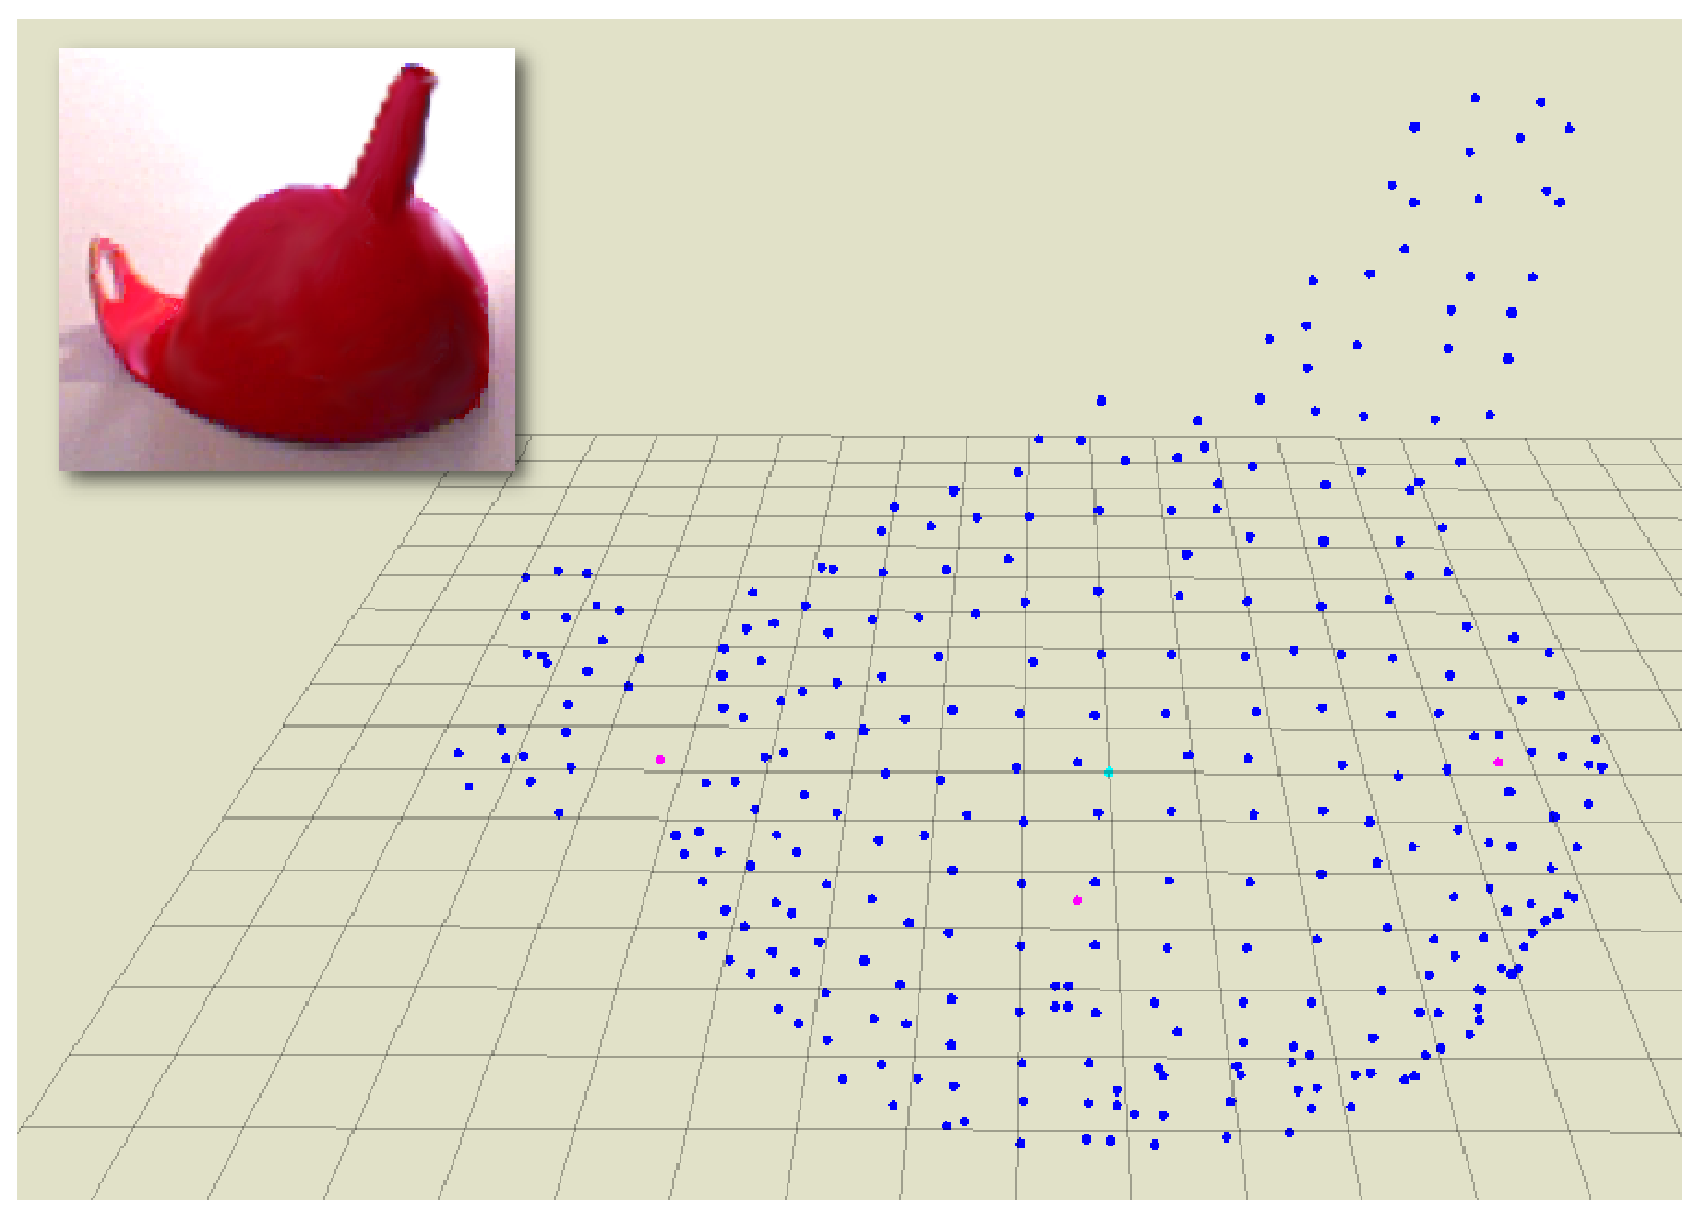
\includegraphics[width=0.45\linewidth]{funnelC.eps}
        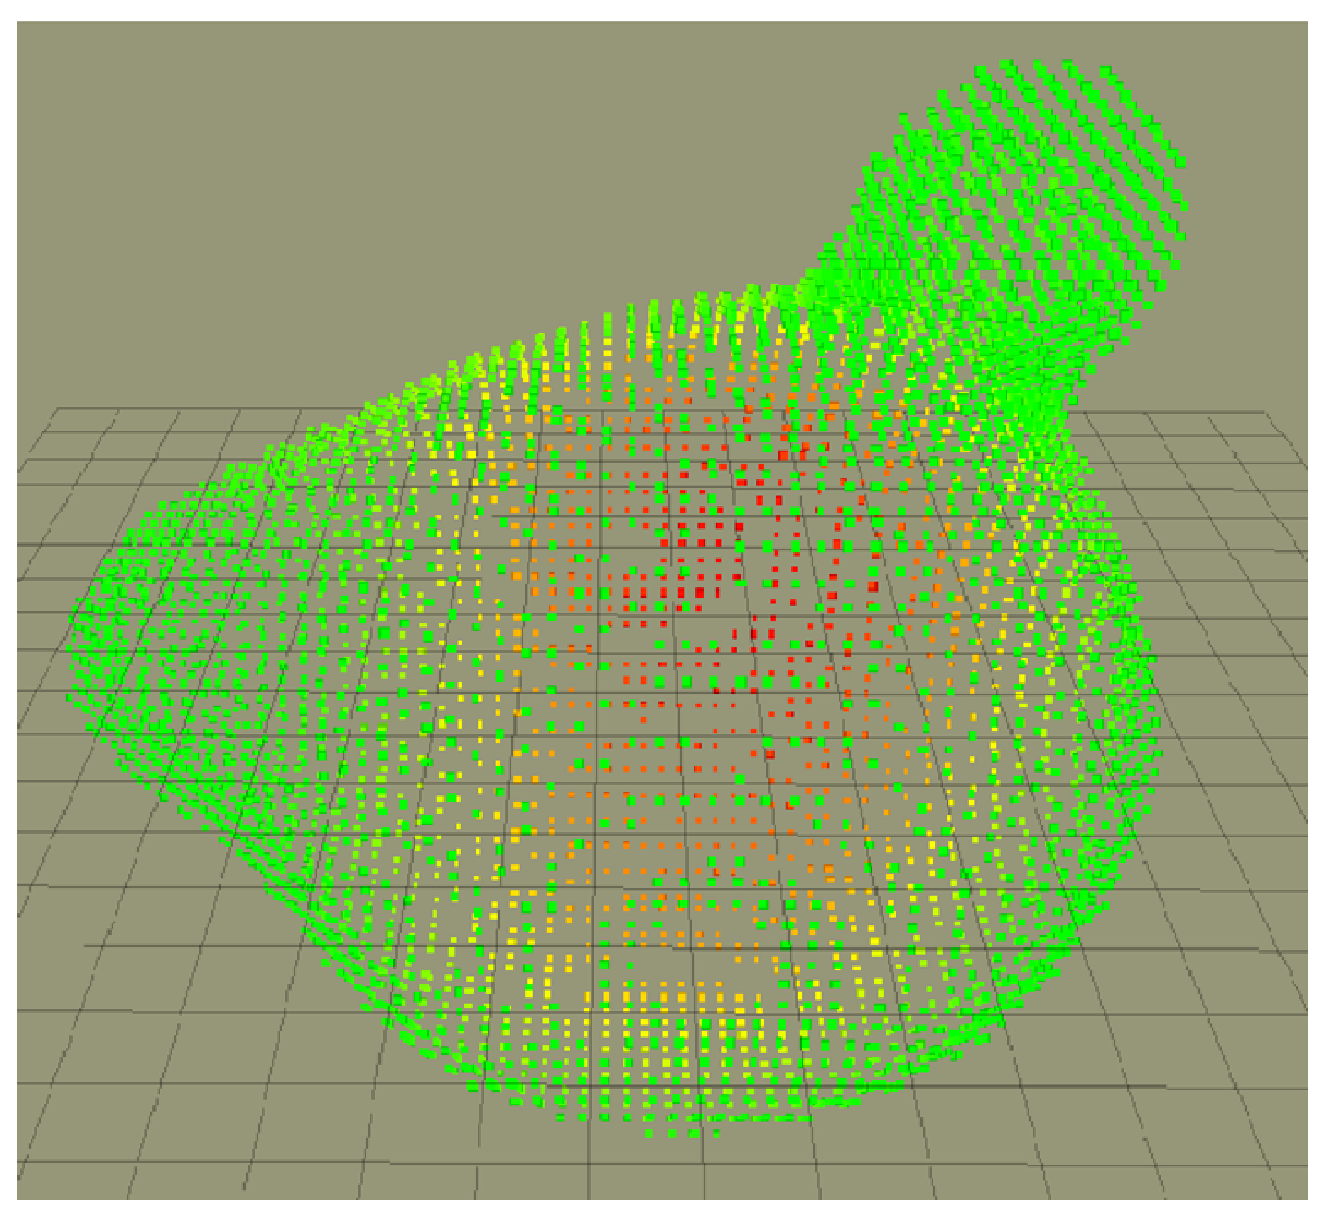
\includegraphics[width=0.45\linewidth]{funnelS.eps}
    }
    \caption{Gaussian Process regression on a funnel object. }
    \label{fig:GPfunnel}
    \todo[inline]{just added to see how it looks on the paper}
\end{figure}
\begin{figure}[h]
    \centering
    \mbox
    {
    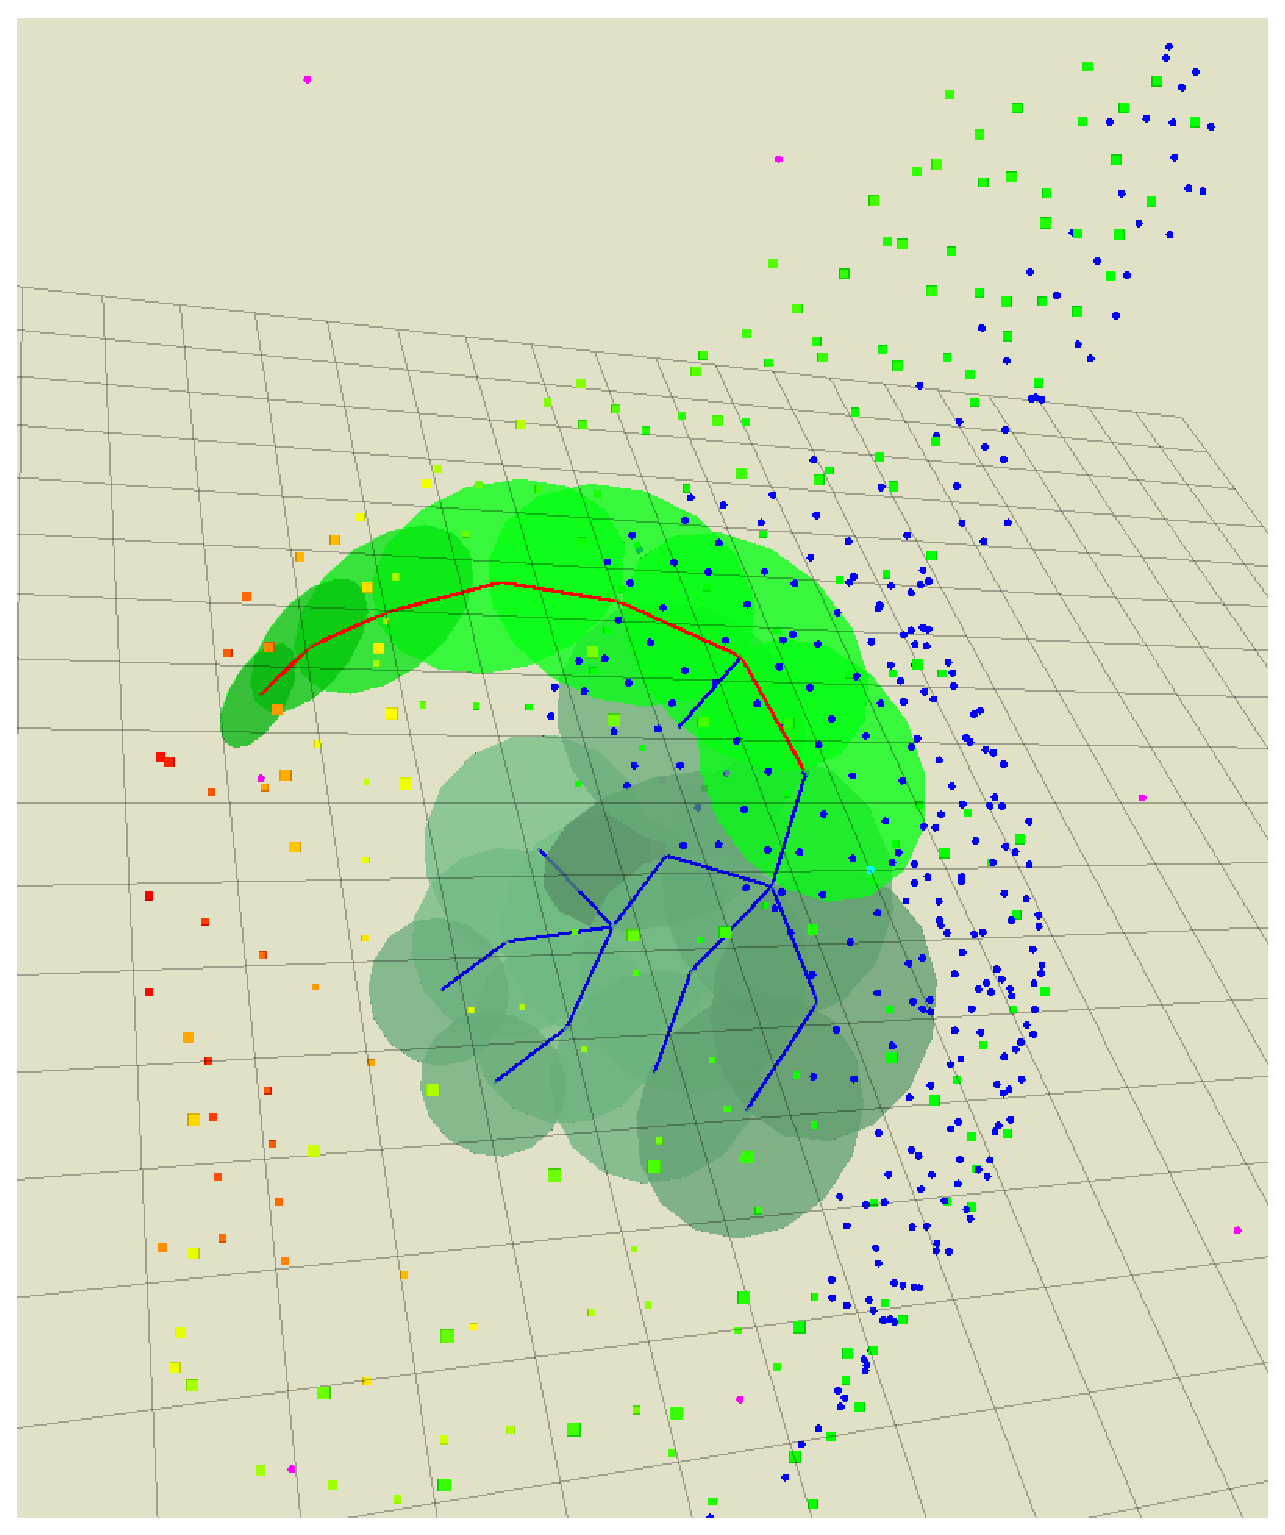
\includegraphics[width=0.45\linewidth]{funnelRRT.eps}
    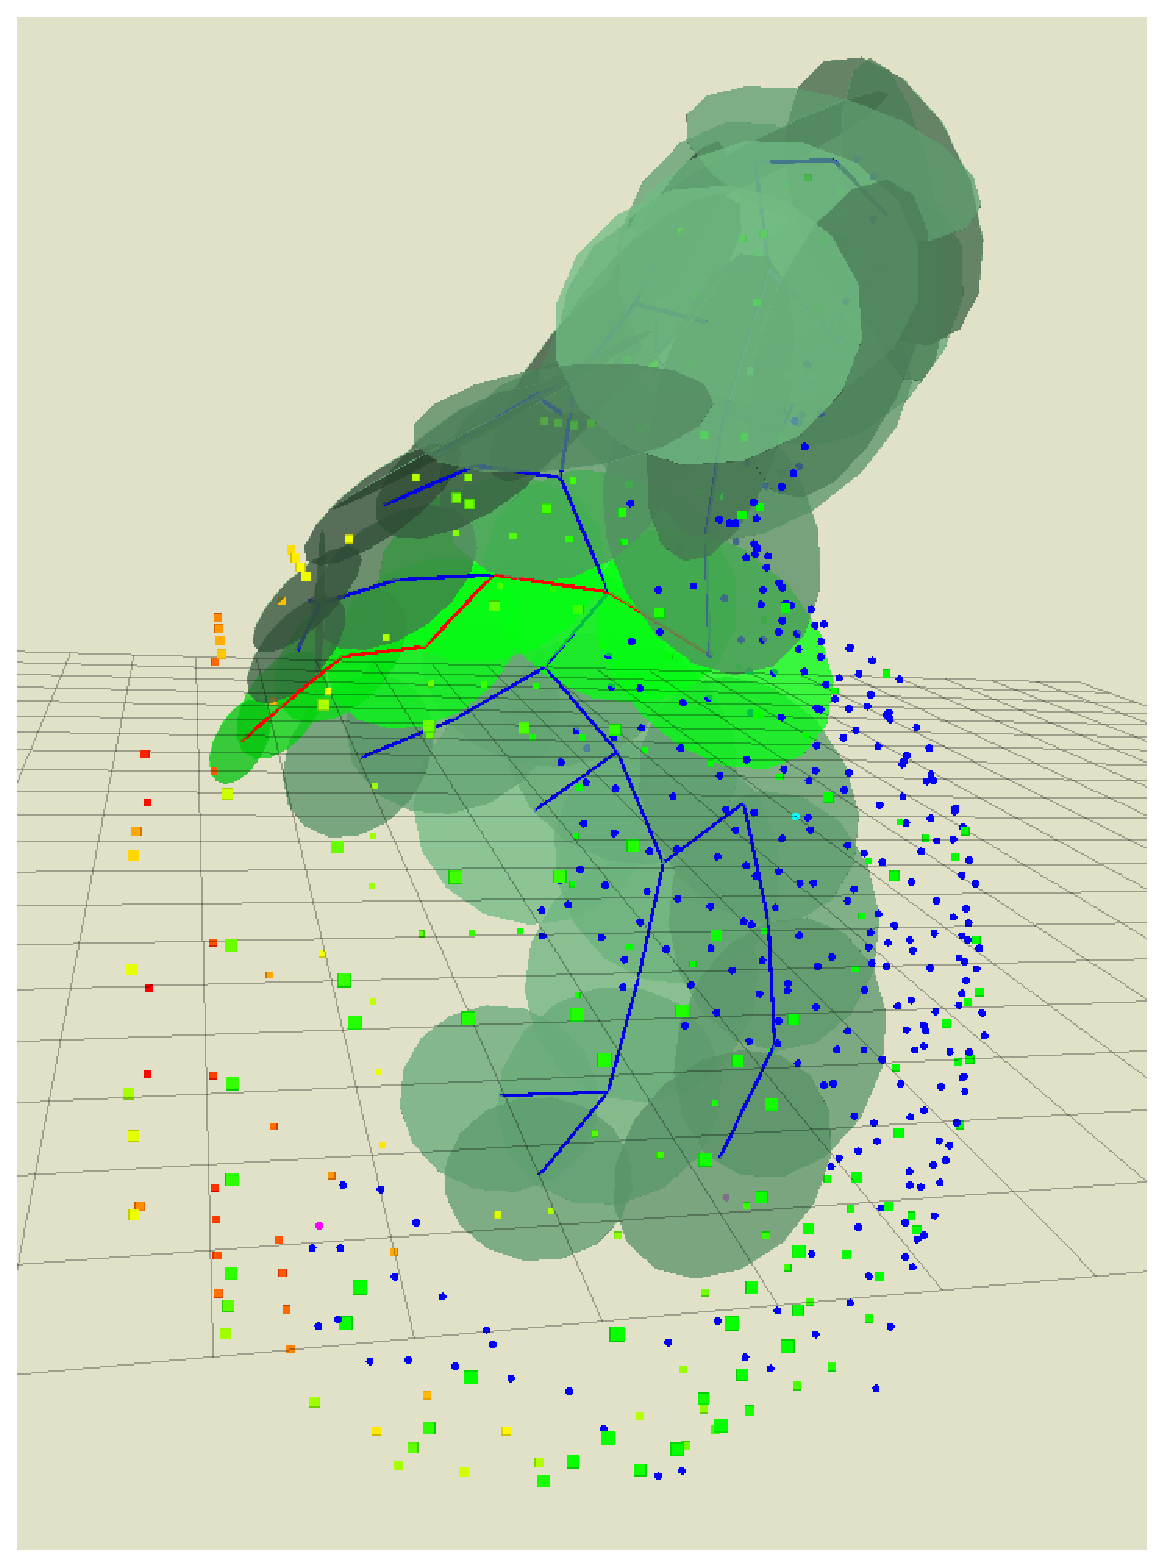
\includegraphics[width=0.45\linewidth]{funnelRRT2.eps}
    }
    \caption{RRT explorer on the funnel implicit surface. Solution is highlighted in green.}
    \label{fig:RRTfunnel}
    \todo[inline]{just added to see how it looks on the paper}
\end{figure}




























%%%%%%%%%%%%%%%%%%%%%%%%%%%%%%%%%%%%%%%%%%%%%%%%%%%%%%%%%%%%%%%%%%%%%%%%%%%%%%%%
\section{The GPAtlasRRT strategy}
\label{sec:solution}

Form the preceding section, probably the reader has envisioned already the dots to connect from both ingredients, the Gaussian process implicit surfaces and the AtlasRRT methodology. The next paragraphs formally describes these connections as the GPAtlasRRT strategy, to give one possible answer to the question raised in the problem statement: an strategy that suggest the best-next tactile exploration candidates to improve the object surface representation, exploiting its probabilistic nature. 

The method starts from an initial and partial observations of the object surface. This is generally provided by vision due to its ability to cope with several points at once. To this end, we assume there is a way to segment the object points out of the scene, that is, points on the object surface\footnote{We provide technical details of our implementation in a real scenario in Subsection~\ref{sec:real}}. However, there could be no information at all, and the probe naively go towards the palm of the gripper holding the object to get a first initial observation, and start from there. As one would expect, this increases the time to get an accurate shape. This initial observations go directly to form the set $\mathcal{S}^0$ to have the object surface model, $\mathcal{GP}$, model provided by (\ref{eq:gp_model}). Since these points are axiomatically on the surface with some degree of uncertainty due the sensor noise, we can compute charts on each of them.
Algorithm \ref{alg:strategy} describes the next-best candidate points for a tactile exploration that to improves input model, $\mathcal{GP}$, up to a predefined variance, $\mathbb{V}_{\max}$. 
The first thing to do is to \textsc{selectSurfacePoint} (line \ref{init}) randomly to get a point $\mathbf{x}_i \in \mathcal{X} \subset \mathcal{S}^0$\footnote{In theory, we can start from all points in the surface, but in practice, this requires too many multi-processes to be properly synchronized}. This is the starting point where the first chart is created, invoking the \textsc{createChart} function (line \ref{create_chart}). The generated data structure contains the center, $\mathbf{x}_i$, the orthonormal tangent basis provided by (\ref{eq:tangent_basis}), $\boldsymbol{\Phi}_i$, note that $\nabla f(\mathbf{x})$ is equivalent to (\ref{eq:gradient_f}), its size, $\rho_i$, and a set of points in the tangent space, $\mathcal{U}_i$. Two things are noticeable here that differentiate us from the original AtlasRRT algorithm. Firstly, the size of a chart, which is a similar to the validity region notion, is inversely proportional to the variance at the chart center, namely,
\begin{equation}
\rho_i \propto \mathbb{V}[f(\mathbf{x}_i)]^{-1}.
\end{equation}
This size is actually the radius of a ball centered at $\mathbf{x}_i$, whose intersection with the tangent space yields \emph{disk}. The motivation behind this choice is that the more certain a point is to be on the surface, the larger the covered region of its chart on the predicted shape, whereas the more uncertain is associated to the center, we prefer to perform smaller exploratory steps.
And secondly, a number proportional to the size of points are sampled uniformly and randomly in the annulus region of the disk with internal and external radius being $0.8\rho$ and $\rho$, respectively. The cardinality of this point-set in the tangent space is proportionally to its size, namely,
\begin{equation}
\#\mathcal{U}_i \propto \rho_i.
\end{equation}
This leads to the fact that the larger the chart, the higher the resolution of directions to expand, hence more samples are needed to have a good quantization of it.
Another advantage of working with a normalized and offset-free set, as mentioned in Subsection \ref{sec:gpis}, is that the parameters that makes the latter two expression to be equalities are tuned once, and remain fixed.

\begin{algorithm}[t]
    \textbf{$\mathcal{P} \leftarrow$ \textsc{GPAtlasRRT}}($\mathcal{M}$, $\mathbb{V}_{\max}$)\\ %functionname
\LinesNumbered
\DontPrintSemicolon
\SetAlgoVlined \SetKwInOut{Input}{input} \SetKwInOut{Output}{output}
\Input{A Gaussian Process model, $\mathcal{M}$ and the set of parameters $\Omega$, defining criteria
    to decide how to start, extend and end the exploration.}
\Output{The best next action, $\mathcal{P}$, in the form of a path, if any, or $\varnothing$ otherwise.}
$\mathbf{x_i} \leftarrow$ \textsc{selectSurfacePoint}($\mathcal{GP}$) \label{init} \\ 
$\mathcal{C}_{i} \leftarrow$\textsc{createChart}($\mathbf{x}_i$, $\mathcal{GP}$) \label{create_chart} \\
% $\mathcal{A}, \mathcal{T}, \mathbf{x}_{c,i} \leftarrow$\textsc{init}($\mathcal{M}$, $\Omega$) \\
$\mathcal{A} \leftarrow$ \textsc{addChart}($\mathcal{C}_i$) \label{add_chart} \\
  \label{is_expandable} \While{ \textsc{isExpandable}($\mathcal{A}$) }
  {
    $\mathcal{C}_j \leftarrow$\textsc{selectChart}($\mathcal{A}$) \label{select_chart} \\
    $\mathbf{x}_k \leftarrow$\textsc{expandChart}($\mathcal{C}_j$, $\mathcal{GP}$) \label{expand_chart} \\
    $\mathcal{C}_k \leftarrow$ \textsc{createChart}($\mathbf{x}_k$, $\mathcal{GP}$) \label{create_new_chart} \\
    $\mathcal{A} \leftarrow$\textsc{addChart}($\mathcal{A}$, $\mathcal{C}_k$) \label{add_new_chart} \\
    \label{ending} \If{ $\mathbb{V}[f(\mathbf{x}_k)]  > \mathbb{V}_{\max}$ }
    {
      $\mathcal{P} \leftarrow$ \textsc{getPath}($\mathcal{C}_i$, $\mathcal{C}_k$) \label{compute_path} \\
      \Return $\mathcal{P}$ \label{return_path} \\
    }
    % \textsc{connect}($\mathcal{T}$, $\mathcal{C}_{k}$, $\mathcal{C}_{j}$) \\
    %$\mathcal{C}_{i} = \mathcal{C}_{k}$ \\
  }
  %\eIf {\textsc{solution}($\mathcal{C}_{i}$)}
  %{\Return $\mathcal{P} \leftarrow$\textsc{path}($\mathcal{C}_{i}, \mathcal{T}$)}
  \Return $\varnothing$ \label{no_candidate}
  \caption{The GPAtlasRRT strategy} \label{alg:strategy}
\end{algorithm}

\begin{figure*}
    \centering
    \mbox
    {
        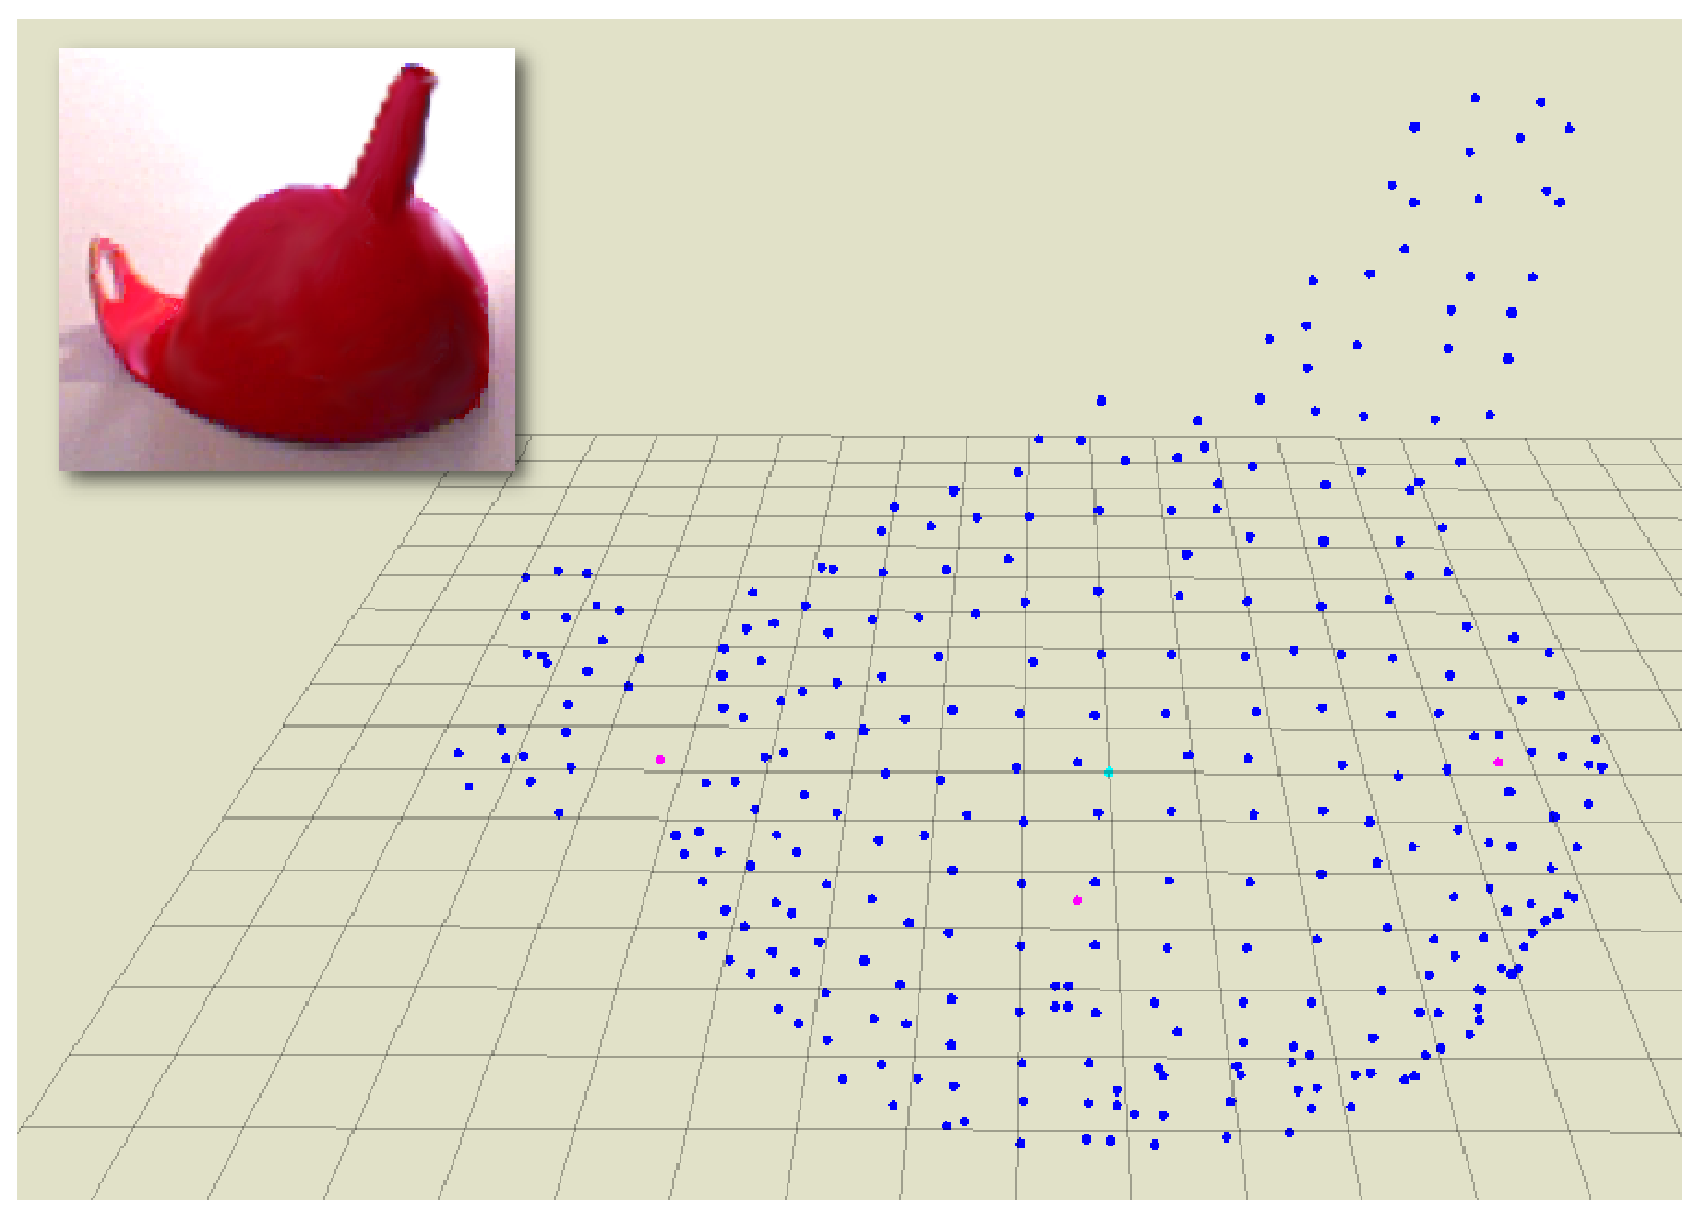
\includegraphics[width=0.33\linewidth]{funnelC.eps}
        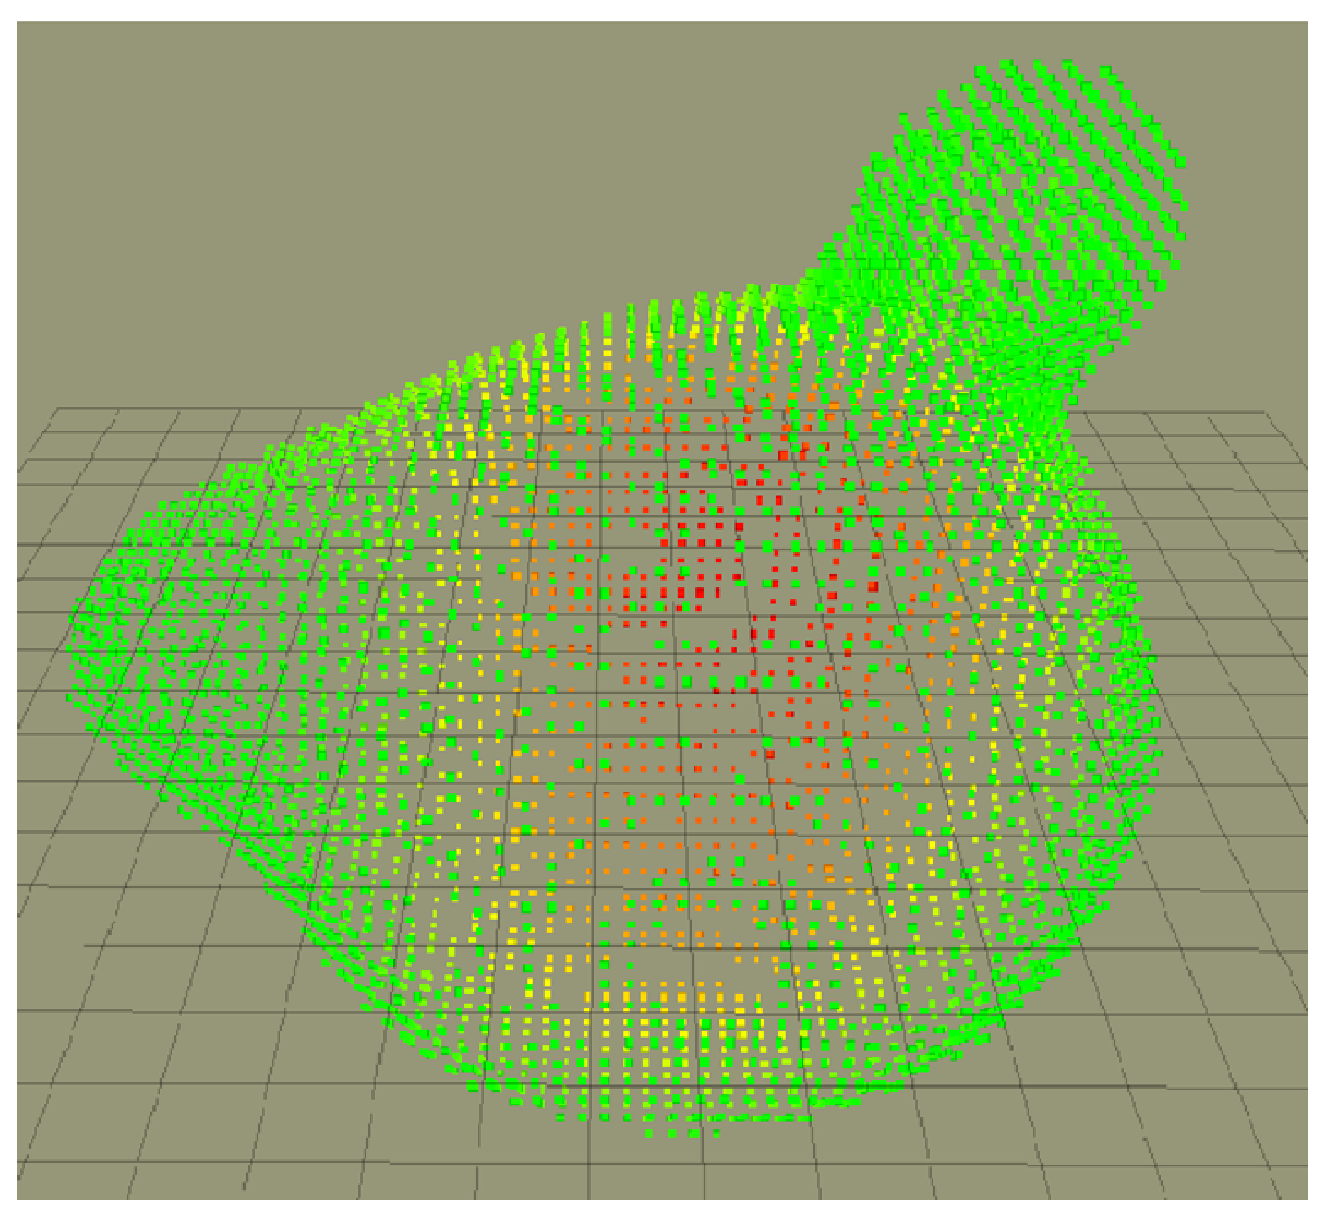
\includegraphics[width=0.33\linewidth]{funnelS.eps}
        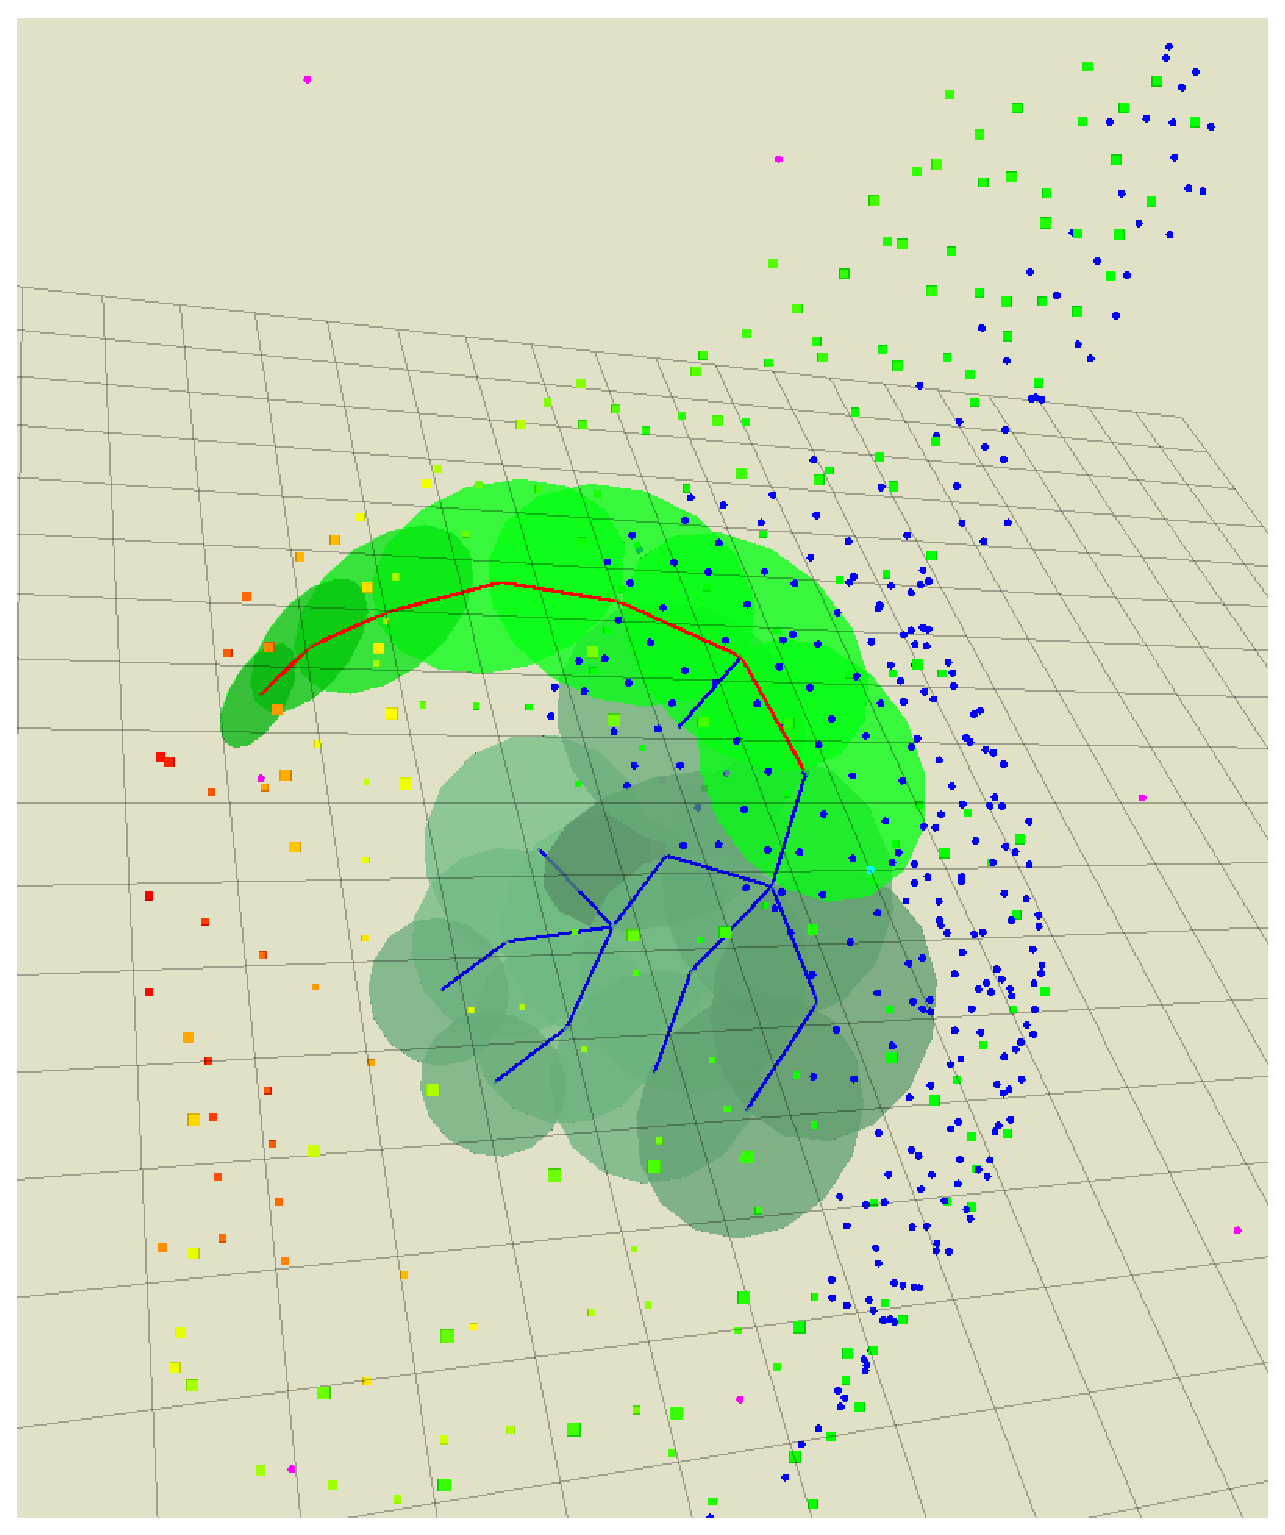
\includegraphics[width=0.33\linewidth]{funnelRRT.eps}
    }
    \caption{ A funnel (left-upper corner) is first seen by a depth camera. The segmented 3D points are sown in blue in the left figure to form the training set $\mathcal{S}^0$. The predicted shape by the GP on this set is shown in the middle obtained via the marching cube algorithm. However, the GPAtlasRRT strategy does not require the explicit form of the predicted surface, as shown in the right figure. It works with the implicit form to devise the next-best tactile exploration shown in brighter green.}
    \label{fig:GPAtlasRRTfunnel}
\end{figure*}

The algorithm continues with the addition of this first chart to the atlas, $\mathcal{A}$, that becomes the root node of an exploration tree (line \ref{add_chart}). The question whether an atlas \textsc{isExpandable} or not (line \ref{is_expandable}) is readily answered by checking whether there is at least one chart with $\#\mathcal{U}_j \neq 0$ or not. The \texttt{false} condition implies that we have covered completely the predicted surface, exiting with no candidate for the best-next tactile exploration (line \ref{no_candidate}). The \texttt{true} condition then makes the flow to continue within the \textbf{while} loop for the iterative exploration. The first step is to \textsc{selectChart} (line \ref{select_chart}) to expand from the atlas. This action takes place randomly among all current charts whose point-set $\mathcal{U} \neq \emptyset$ using a trade-off proportion between depth-first (or selecting the previously expanded chart with probability $p = 0.4$) and breadth-first (or selecting any other chart with probability $1-p$) for the tree expansion. Note that, in the first iteration, $\mathcal{C}_i$ is the only one, and it is surely expandable. Next, the \textsc{expandChart} operation on the selected chart (line \ref{expand_chart}) chooses among all points $\mathbf{u}_{j,t} \in \mathcal{U}_i$, the one with the largest variance in ambient space, that is,
\begin{equation}
\mathbf{u}_{j}^* =  \argmax_{\mathbf{u}_{j} \in \mathcal{U}} \mathbb{V}[f(\phi_j(\mathbf{u}_{j}))], 
\end{equation}
where the tangent basis approximation of the mapping $\phi_j(\cdot)$ is used as given in (\ref{eq:tangent_approx}). The point $\mathbf{x}_k^j = \phi(\mathbf{u}_{j}^*)$ is then projected to the predicted surface solving (\ref{eq:projection}), as mentioned, using a gradient-descent-like method to obtain the point $\mathbf{x}_k \in \mathbf{X}$. A chart, $\mathcal{C}_k$, is then created from this point and added to the current atlas (lines \ref{create_new_chart}--\ref{add_new_chart}). When a new chart is added to the atlas, all sets $\mathcal{U}$ of all charts are reduced by discarding the points that fall within the validity region of other charts existing in the atlas. This was not mentioned in the first call of the \textsc{addChart} in line \ref{add_chart}, because at that point there is only the root chart in the atlas. Finally, the expected variance of the center of the last chart added is compared against the input parameter $\mathbb{V}_{\max}$ (line \ref{ending}). The \texttt{false} condition of the \textbf{if} statement makes the algorithm to continue with the atlas expansion, whereas the \texttt{true} condition return the next-best exploration path, $\mathcal{P}$ (lines \ref{compute_path}--\ref{return_path}). Recall that this path is in the predicted shape of the object, therefore the control to follow it must be compliant to avoid damages. The new tactile observations tells whether the predicted shape is good or not by increasing the training set, $\mathcal{S}^0$, to automatically reduce the variance along the path, and improve the overall uncertainty of surface model. The next section traces how the GPAtlasRRT strategy can be embedded in a tactile exploration scenario.

\subsection{Tactile exploration for object surface modeling via the GPAtlasRRT strategy}
\label{sec:gpatlasrrt_tactile_exploration}

Algorithm~\ref{alg:solution} presents the pipeline model of a tactile exploration to model the surface of an object driven by the GPAtlasRRT strategy. As anticipated in the previous section, the initial and partial observation can be taken from visual input or a naive probe (lines to compute the model \ref{ini_gp}--\ref{fini_ini_gp}). From this point on, we plan the next-best tactile exploration, $\mathcal{P}$, (line \ref{exploration}), and pass this information to the exploratory probe. Please, note that this exploration can done by a real robot or simulated given a ground truth, a notion that is used for the method validation in Section \ref{sec:experiments}.

Thus, the exploratory probe system \textsc{approachTo} the exploration path, typically to the first point with low uncertainty when \emph{sliding} or to the final point with high uncertainty when \emph{poking} with the goal being a safety distance away from the predicted surface in the direction normal at the corresponding point. This phase can be done with a position control scheme and collision avoidance motion planning. The latter is an interesting topic, since the object shape is not known. But it can be predicted with the current state of the model to some degree of uncertainty. A coarse point cloud can be computed out of the model and build a probabilistic collision map based on the expected variance of the function values at the point cloud. Next, we proceed to \textsc{probeObject} following the next-best path, $\mathcal{P}$, to get observations of points being on or outside of the surface, and labeled accordingly altogether in the exploration log set, $\mathcal{S}^{0+}$ (line \ref{probe}). In this phase, the collision avoidance motion is disable and the probe moves compliantly, like in a contour-following set-up, and uses the tactile sensing to detect whether the probe is contacting or not with the object surface. Once the end of the path is reached, the training set is accordingly updated keeping the old training set, and applying the normalization and offset-free operations after the addition of new data (line \ref{update_training}). This is then used to recompute a better model of the object surface, $\mathcal{GP}$ (line \ref{re-compute}). Simultaneously (using the old model) or afterwards (using the updated model), we engage again the position control and collision avoidance motion planning to take the exploratory probe to its rest position (line \ref{away}). When the \textsc{GPAtlasRRT} returns an empty path, $\mathcal{P} = \varnothing$, then we say that the predicted shape by the returned model, $\mathcal{GP}$, has at most a variance of $\mathbb{V}_{\max}$ for any point on the surface, that is, $\mathbb{V}[f(\mathbf{x})] < \mathbb{V}_{\max}, \, \forall \mathbf{x} \in \mathcal{X}$.

\begin{algorithm}[t]
\textbf{\textsc{TactileExploration}}($\mathcal{Z}, \mathbb{V}_{\max})$\\ %functionname
\LinesNumbered
\DontPrintSemicolon
\SetAlgoVlined \SetKwInOut{Input}{input} \SetKwInOut{Output}{output}
\Input{An initial point cloud of the scene, $\mathcal{Z}$, and the desired variance, $\mathbb{V}_{\max}$, for the overall surface prediction.}
\Output{The object model as a Gaussian process, $\mathcal{GP}$.}
  \label{ini_gp} \If{ \textsc{isEmpty}($\mathcal{Z}$ }
  {
    $\mathcal{S}^0 \leftarrow $ \textsc{naiveProbe}() \\
  }
  \Else
  {
    $\mathcal{S}^0 \leftarrow $ \textsc{segmentObject}($\mathcal{Z}$) \\
  }
  $\mathcal{S} \leftarrow$ \textsc{generateTrainSet}($\mathcal{S}^0$)
  $\mathcal{GP} \leftarrow $\textsc{computeModel}($\mathcal{S}$) \label{fini_ini_gp} \\
  \While { \texttt{true} } 
  {
    $\mathcal{P} \leftarrow $\textsc{GPAtlasRRT}($\mathcal{GP}, \mathbb{V}_{\max})$ \label{exploration} \\
    \If{ $\mathcal{P} \neq \varnothing$ }
    {
      \textsc{ApproachTo}($\mathcal{P}$, $\mathcal{GP}$) \label{approach} \\
      $\mathcal{S}^{0+} \leftarrow $\textsc{probeObject}($\mathcal{P}$) \label{probe} \\
      %$\mathcal{S}^0 \leftarrow$ \textsc{getOnSurface}($\tilde{\mathcal{S}^{0+}}$) \\
      %$\mathcal{S}^+ \leftarrow$ \textsc{getOutsideSurface}($\tilde{\mathcal{S}^{0+}}$) \\
      $\mathcal{S} \leftarrow$ \textsc{updateTrainSet($\mathcal{S}$, $\mathcal{S}^{0+}$)} \label{update_training} \\
      $\mathcal{GP} \leftarrow $\textsc{computeModel}($\mathcal{S}$) \label{re-compute} \\
      \textsc{MoveAway}($\mathcal{GP}$) \label{away} \\
    }
    \Else
    { 
      \Return {$\mathcal{GP}$} \label{solutionfound} \\
    }
  }
\caption{Surface modeling via GPAtlasRRT} \label{alg:solution}
\end{algorithm}

%\subsection{Probabilistic completeness}
%\label{sec:reasoning}

%First of all, we can safely assume that the surface of any household object is a $1$-component manifold.








% During the \textsc{ApproachTo} (line~\ref{approach}) (\textsc{MoveAway}, line~\ref{away}) phases, the robot uses position control and standard motion planning techniques with collision avoidance. Since we are modelling the shape, we need to ensure that everytime the robot moves close (away) from the object, it does not collide with the object. It is tentative to use the current estimated shape, but since we are not actually computing it explicitly in our approach, we choose the bounding sphere as the collision geometry of the object. Thus the robot moves towards (away from) the surface at the contact location in the normal direction until reaching the bounding sphere. After that, a standard motion planning is used to approach the object (get to the rest position).

% The \textsc{probeObject} (line~\ref{probe}) phase is engaged once the robot is within the bounding sphere. The robot uses Cartesian impedance control, with the Cartesian force, pose and impedance set properly for the given setup. These implementation details are given in the next section. Since we don't actually know where the surface is, we need to whether the robot actually touched something or not, in order to properly label the acquisition (lines~\ref{belonglabel} and~\ref{nobelonglabel}) 

% The method finishes when \textsc{exploreGPAtlasRRT} (line~\ref{exploration}) described in Algorithm~\ref{algo:strategy} has explore sufficiently the estimated shape and could not find an exploratory action $\Gamma$ (line~\ref{solutionfound}), i.e. the object shape is probabilistically estimated within the 95\% of the confidence interval computed from $\mathbb{V}_{des}$. 

%The complete solution of the problem as stated in~\ref{sec:scope} is depicted in Algorithm~\ref{alg:solution}.



%This section provides a more detailed description of our GPAtlasRRT algorithm. As described in Sec.~\ref{sec:scope}, our approach combines probabilistic inference on an unknown surface with a asymptotically optimal sample-based exploration technique for implicitly-defined configuration spaces (manifolds). We demonstrate the efficiency of our proposed solution in a bimanual framework (see Sec.~\ref{sec:scenario}) where a humanoid robot (Vito) can hold an unknown object in one hand and actively build up a probabilistic model of the object's shape by integrating visual and haptic information. This is done efficiently by selecting haptic actions which lead to an asymptotically optimal reduction of the global shape uncertainty of the model. 

%We employ a GP to learn a probabilistic model of the object surface, encoded as an implicit surface, constrained to visual and tactile clues iteratively acquired. First we rely on visual information captured by a RGB-D camera, which will be pre-processed, as described in Sec.~\ref{sec:segmentation}, to isolate the object's point cloud from the rest of the scene (robot's and environment's). Secondly we generate artificial points to improve the performance of the GP estimation, and after having labelled them properly we pass them as training inputs to the GP procedure. This procedure will be described in Sec.~\ref{sec:shape}. 

% The (noisy) visual observations constrain our model which has the effect of increasing its confidence (reduced variance) on its predictions about the function value $f(\mathbf{x})$ in regions highly populated by the training dataset. However, predictions in occluded or unseen regions will be associated with lower confidence (high uncertainty) since few or none information are available.  

% To improve the accuracy of our model, we make inference on it to build paths along the estimated object's surface such that a robot finger equipped with F/T sensors can collect haptic information over unseen regions of the surface. Since the surface is encoded as an implicit surface we need a more efficient way to make inference than to just attempt to reconstruct the expected object's shape via a highly-dense randomly generated samples. Instead we utilise the notion of manifold as a collection of local parametrisation (charts) such that we can make predictions on the neighbouring regions of already visited points as well as generate more charts on the more recent visited regions. To keep track of how the charts are generated and connected by themselves, we employ an RRT-like algorithm to build a tree of charts. The algorithm terminates when a path to a region, which is more promising to reduce the overall shape uncertainty of our model, is found.

%Section~\ref{sec:strategy} will explain the novelty of our algorithm in detail.  


% \begin{algorithm}[h]
% \textbf{\textsc{createGaussianProcess}}($X$)\\ %functionname
% \LinesNumbered
% \DontPrintSemicolon
% \SetAlgoVlined \SetKwInOut{Input}{input} \SetKwInOut{Output}{output}
% \Input{The training data, $\mathcal{X}$, in the form of a point cloud.}
% \Output{The Gaussian Process that models the object shape.}
%   $\mathcal{D} \leftarrow$\textsc{deMeanNormalizeAndLabel}(\{$\mathcal{X}$, $\mathbf{0}_{\text{sizeOf}(\mathcal{X})}$\}) \\
%   \textsc{addLabeledPoint}(\{$\mathbf{0}_3, -1\}$, $\mathcal{D}$) \\
%   \textsc{addLabeledPoints}(\{\textsc{sphere}$(\mathbf{0}_3, 1.1, N)$, $+\mathbf{1}_{N}\}$, $\mathcal{D}$) \\
%   $\mathcal{G} \leftarrow$ \textsc{doRegression}($\mathcal{D}$) \\
%   \Return $\mathcal{G}$ \\
% \caption{Gaussian Process regression} \label{algo:strategy}
% \end{algorithm}

%%%%%%%%%%%%%%%%%%%%%%%%%%%%%%%%%%%%%%%%
%\subsection{Best-next tactile strategy}
%\label{sec:strategy}

%Algorithm~\ref{alg:strategy} presents a pseudo-code of our implementation. As previously described in Sec.~\ref{sec:scope}, we explore the estimated surface of the object via a combination of probabilistic inference and sample-based techniques for manifolds. 

%We employ an RRT-like algorithm which, instead of growing in the ambient space, is embedded in an implicitly defined configuration space defined by a manifold or Atlas, $\mathcal{A}$. The major difference between our proposed implementation and a traditional RRT-algorithm is in how we select a new candidate node and expand the tree.


%
%The RRT explorer, however does not have any information on the model on which is built, specifically,
%it just need to track the connections between nodes of the tree and decide where it
%should expand next. All the model information is stored in an Atlas, called $\mathcal{A}$.
%
%An atlas can be viewed as a collection of maps or charts and conceptually it is able
%to create new charts at a given location on the surface it is currently modelling.
%Furthermore $\mathcal{A}$ is able to expand a given chart, producing new locations
%from where create new charts.
%
%In the proposed exploration strategy, RRT nodes are exactly the charts, thus
%building such a tree is like composing an atlas, which tries to model the implicit
%estimated surface.
%
%Formally we define a chart $\mathcal{C}$ with a center point on the surface $\mathbf{x}_{c}$,
%such that
%$$
%\mathbb{E}(\mathcal{S}(\mathbf{x}_c)) \approx 0
%$$
%with a search space defined as a
%tangent disc at the surface, centered on $\mathbf{x}_c$, with radius 
%$$
%R \propto \frac{1}{\mathbb{V}(\mathcal{S}(\mathbf{x}_c))}
%$$ 
%and finally with the gradient information at the center 
%$$
%G \approx \frac{\partial \mathcal{S}}{\partial \mathbf{x}}
%$$
%Conventionally the center variance is addressed as the chart variance, because
%it locally approximates the uncertainty of the surface estimation.
%
%With such charts, the atlas can be defined as the set of all charts plus some parameters
%responsible for chart creation:
%$$
%\mathcal{A} \triangleq \{\mathcal{C}_1, \ldots, \mathcal{C}_i, \ldots, \mathcal{C}_n, \Omega^{\mathcal{A}}\}
%$$
%where $n$ is the number of created charts and $\Omega^{\mathcal{A}}$ are the parameters.
%
%The explorer can also be viewed as a collection of chart connections, or branches,
%plus another set of parameters responsible for the tree expansion behaviour:
%$$
%\mathcal{T} \triangleq \{\mathcal{C}_i \leftarrow \mathcal{C}_j, \ldots, \Omega^{\mathcal{T}}\}_{i \neq j \le n}
%$$



%Given a Gaussian Process model, $\mathcal{M}$, approximating the implicit object surface
%with a regression, as described in Sec.~\ref{sec:gpr}, and the set of parameters
%$$\Omega \triangleq \Omega^{\mathcal{A}} \cup \Omega^{\mathcal{T}}$$
%An empty atlas and a RRT explorer can be initialized.
%Then a starting point is selected randomly among the object training set:
%$$
%\mathbf{x}_{c,i} \in \chi^0
%$$
%where $\chi^0$ is the set of object points,
%which in turn is part of the Gaussian Process Model, $\mathcal{M}$.
%
%$\mathcal{A}$ is charged to create the first chart, also called \emph{root}, from the starting point,
%then the algorithm rapidly builds the tree of charts on the object until the supplied termination
%criterion is met, or the maximum allowed number of charts has been reached.
%The best-next tactile action is finally the path from the converging chart to the root, or nothing if no such chart exists.

%The main loop of the algorithm is fulfilled by the following steps:\\
%\begin{inparadesc}
%\item[select($\cdot$)] Ask the explorer to select a chart to expand,
%among the chart collection ($\mathcal{A}$).
%This is done by selecting one at random with a bias to increase the probability
%of selecting the last created chart. This criterion is adopted to grow a tree
%which is more inclined to expand on a single branch, but at the same time maintain the
%possibility to create new branches from previous charts. So efficiency and speed
%is preserved, while we make sure we are exploring as much surface as possible,
%before reaching a solution.\\
%\item[expand($\cdot$)] The selected chart $\mathcal{C}_j$ is expanded by $\mathcal{A}$, by
%sampling $k$ points on its tangent discs then selecting one at maximum variance
%and at the same time not in collision with other charts search spaces. 
%So a sample $\mathbf{s}_i$ is selected if 
%$$
%\mathit{max}_{i\in k}[\mathbb{V}(\mathcal{S}(\mathbf{s}_i))]
%$$
%and 
%$$
%{\parallel\mathbf{s}_i - \mathbf{x}_{c,j}\parallel}_{2} > R_j, \forall \mathcal{C}_j \in \mathcal{A}_{i \ne j}
%$$
%where $\mathbf{x}_{c,j}$ is the center and $R_j$ is the tangent disc radius of $\mathcal{C}_j$.

%The selected $\mathbf{s}_i$ is then projected back on the surface,
%creating a center for a new chart, $\mathbf{x}_{c,k}$.
%The projection is performed with a gradient descend method, using the gradient estimation
%of the chart $G_j$.\\
%\item[create($\cdot$)] A new chart  is created on the projected point, maintaining the atlas
%    expansion on the estimated implicit surface
%$$
%\mathcal{C}_k \in \mathcal{A}
%$$
%\item[connect($\cdot$)] creates a connection to the chart which originated the newly created one,
%    drawing a new branch for the tree
%$$
%\{\mathcal{C}_j \leftarrow \mathcal{C}_k \} \in \mathcal{T}
%$$
%\end{inparadesc}

%$\mathcal{C}_k$ is then tested for the termination condition and the whole loop
%starts anew.

%The progressively growing tree of charts expands on the object surface until
%the termination criterion is met. Then, when this happens, the procedure terminates and the full
%path from the converging chart to the root of the tree is reported as a solution.

%Furthermore, to customize the exploration, the parameters in $\Omega^{\mathcal{A}}$ 
%control how much chart search spaces are big according to their variances and how many
%samples are generated during the \textsc{expand}($\cdot$) phase. 
%We chose to create tangent disc radii inversely proportional to their variance,
%because, when the uncertainty/variance is low, we want to expand further
%away from the starting chart, traversing reasonably certain surfaces faster.
%On the contrary, when the uncertainty/variance is high, we want to make small
%exploration steps, because we are not certain of the underlaying estimated surface.

%We chose to have a variance threshold as a termination condition, defined in $\Omega^{\mathcal{T}}$,
%because when the exploration reaches a chart with high variance, we want to stop
%the exploration and perform a tactile action there to reduce the uncertainty in the
%model. 
%% The action will bring new data to update the shape estimation and eventually 
% a new more accurate exploration can be started with updated model.

%%%%%%%%%%%%%%%%%%%%%%%%%%%%%%%%%%%%%%%%%%%%%%%%%%%%%%%%%%%%%%%%%%%%%%%%%%%%%%%%
\section{Validation and experiments}
\label{sec:experiments}

%\subsection{Validation of the methodology}

% \subsection{Testing is simulated scenario}\label{sec:synth}
In order to validate our algorithms we devised a simulated touching environment,
where we performed a number of tests on 9 everyday objects, like bowls, pots, spoons and mugs.
In order to have a ground truth for our tests we used complete point clouds and polygonal meshes of
such objects, shown in Figure~\ref{fig:meshes}.

\begin{figure}[htb]
    \centering
    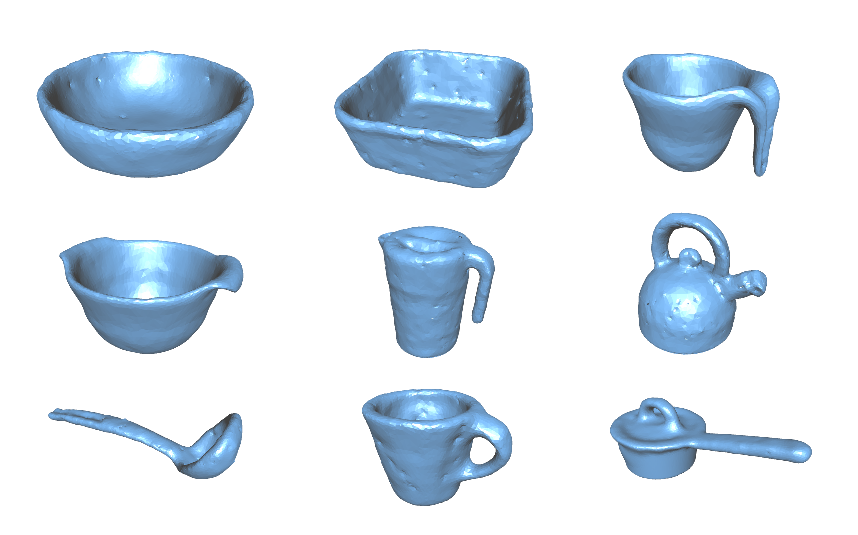
\includegraphics[width=0.95\columnwidth]{meshes.eps}
    \caption{Object meshes used as ground truth for our tests. From top to bottom and from left
    to right: bowlA, bowlB, containerA, containerB, jug, kettle, spoon, mug and pot.}
    \label{fig:meshes}
\end{figure}

These data represent full reconstructed shapes and were obtained by means of a common RGBD sensor and a turn table. The meshes created this way are used as ground truth comparison for shapes reconstructed by our algorithm and at the same time, are used to extract partial view point clouds to set as initial training data ($\mathcal{S}^0$), for our Gaussian Process regression, see Sec.~\ref{sec:gpis}.
It is worth nothing, that the meshes obtained this way are affected by sensor measurement noise 
and they don't perfectly represent the real object shapes. However this is no concern for us, because also the
training sets used in our validation are obtained from the same meshes, thus estimation and ground truth are
consistent with each other.

Each test we performed encloses a full object shape reconstruction and it's carried over
by iterating our \textsc{GPAtlasRRT} algorithm, Alg.~\ref{alg:strategy}~in~Sec.~\ref{sec:solution},
until the shape is predicted with desired variance $\mathbb{V}_{\max} = 0.1$.
% find a solution path that defines the best next tactile action to perform, until

The best tactile action to perform at each iteration is simulated in our
environment by using  raycasting techniques towards the ground truth mesh.
Rays are uniquely defined by a chart center, as pivot point, and its normal, as direction.
Thus we can define  ray-mesh intersections as touches, i.e. points on surface, and no intersections
as points outside the surface. These new points are used to update the training set
and the GP model, from which a new \textsc{GPAtlasRRT} iteration can take place. 

In order to broaden our tests, we adopted three different tactile actions for each object, consequently forming 
three test groups, for a total of 27 full shape reconstructions. Each test group is described as follows:
\begin{asparadesc}
    \item[Random Touch], for the first test group we ignored the \textsc{GPAtlasRRT} solution path and 
        we just touched a random point on the GP manifold, with the raycasting technique described above.
        The random touching is repeated until the reconstructed shape is correctly predicted with
        maximum variance of $0.1$.
        It is worth nothing that we expected these tests to take a large number of touches
        in order to reconstruct the shape and they were performed as a comparison for our method.
        Test results are visible in Table~\ref{tab:test1}.
    \item[Single Poking], for the second test group we actually begin using the \textsc{GPAtlasRRT} solution by
        poking the last chart identified by the path, i.e.\ we used the raytracing technique applied to the last
        chart of the solution path, performing a touch where the algorithm recommends.
        Convergence criteria are the same as the previous test, thus we repeat tactile actions
        until the shape is fully reconstructed. Results in Table~\ref{tab:test2} show a significant reduction
        in number of tactile actions required, in order to reach the requested shape variance.
    \item[Sliding Touch],  for the  final test  category we  decided to use the
    \textsc{GPAtlasRRT}  full solution  path. Starting from the root chart we begin raytracing towards the ground truth mesh and from the touched point we
    re-interpolate a  path towards the next  chart. The new path  is raycast
    again, while it is being traversed, yielding another point to generate a new interpolated path, and so
    on until we traverse all the charts in the path and we reach the tip of the atlas branch.
    With this technique we mimic a probe that is trying to slide across the surface,
    while trying to maintain contact with it. As the virtual probe slides we can discover
    a fairly significant amount of points on the surface and thus we can add more points to the training set
    with a single action. For this very reason we expected this test to be the highest performing among the three,
    in terms of step requirements, but also in terms of the quality of the reconstructed shape.
    Table~\ref{tab:test3} shows this test result, which met our expectations.
\end{asparadesc}
\begin{table}
    \centering
    \begin{tabularx}{0.95\columnwidth}{lccccccr}
        \toprule
        Object &&& & & Steps && RMSE \\
        \midrule
        bowlA &&& & &67 && 0.0025\\
        bowlB &&& & &38 && 0.0038\\
        containerA &&&&& 124 && 0.0033\\
        containerB &&&&& 68 && 0.0062\\
        jug &&&&& 106 && 0.0027\\
        kettle &&&&& 98 && 0.0031\\
        spoon &&&&& 35 && 0.0058\\
        mug &&&&& 238 && 0.0017\\
        pot &&&&& 33 && 0.0035\\
        \midrule
        \textbf{Mean} &&&&& $\sim$\textbf{90} && \textbf{0.0036}\\
        \bottomrule
    \end{tabularx}
    \caption{Random Touch test results in terms of the required
    number of actions (Steps) and the Root Mean Squared Error (RMSE) between
    the predicted shape and the ground truth mesh.}
    \label{tab:test1}
\end{table}
\begin{table}
    \centering
    \begin{tabularx}{0.95\columnwidth}{lccccccr}
        \toprule
        Object &&& & & Steps && RMSE \\
        \midrule
        bowlA &&& & &27 && 0.0023\\
        bowlB &&& & &18 && 0.0036\\
        containerA &&&&& 20 && 0.0035\\
        containerB &&&&& 19 && 0.0043\\
        jug &&&&& 20 && 0.003\\
        kettle &&&&& 17 && 0.0032\\
        spoon &&&&& 10 && 0.0055\\
        mug &&&&& 28 && 0.0020\\
        pot &&&&& 12 && 0.0032\\
        \midrule
        \textbf{Mean} &&&&& $\sim$\textbf{19} && \textbf{0.0034}\\
        \bottomrule
    \end{tabularx}
    \caption{Single Poking test results in terms of the required
    number of actions (Steps) and the Root Mean Squared Error (RMSE) between
    the predicted shape and the ground truth mesh.}
    \label{tab:test2}
\end{table}
\begin{table}
    \centering
    \begin{tabularx}{0.95\columnwidth}{lccccccr}
        \toprule
        Object & & &&& Steps && RMSE \\
        \midrule
        bowlA &&& & &8 && 0.0015\\
        bowlB & &&& &5 && 0.0028\\
        containerA &&&&& 11 && 0.0028\\
        containerB &&&&& 8 && 0.0026\\
        jug &&&&& 9 && 0.0025\\
        kettle &&&&& 9 && 0.0029\\
        spoon &&&&& 8 && 0.0031\\
        mug &&&&& 12 && 0.0018\\
        pot &&&&& 6 && 0.0028\\
        \midrule
        \textbf{Mean} &&&&& $\sim$\textbf{8} && \textbf{0.0025}\\
        \bottomrule
    \end{tabularx}
    \caption{Sliding Touch test results in terms of the required
    number of actions (Steps) and the Root Mean Squared Error (RMSE) between
    the predicted shape and the ground truth mesh.}
    \label{tab:test3}
\end{table}

The three experiments clearly show the superiority of our method in terms of number of required steps
and in terms of quality of the produced mesh. As a final benchmark, Table~\ref{tab:comp} summarizes the comparison
between the test methods and Fig.~\ref{fig:shapecomp} shows some  of the \textsc{GPAtlasRRT} Sliding Touch reconstructed shapes with
the ground truth meshes next to them.
\begin{table}
    \centering
    \begin{tabularx}{0.95\columnwidth}{lccccr}
        \toprule
        Tests  &&& Mean Steps && Mean RMSE \\
        \midrule
        Random Touch & & &90 && 0.0036\\
        Single Poking && &19 && 0.0034\\
        Sliding Touch &&& 8 && 0.0025\\
        \bottomrule
    \end{tabularx}
    \caption{Overall comparison: GPAtlasRRT with Sliding Touch outperforms in terms
    of efficiency and accuracy.}
    \label{tab:comp}
\end{table}


Additionaly, while we performed our validation, we also recorded some videos of shape reconstructions, visible online at \texttt{goo.gl/4GKYTp}.

\vspace{-2em}
\subsection{A real tactile exploration}
\label{sec:real}

The purpose of this test is to illustrate with an example an implementation of Algorithm \ref{alg:solution}. However, as mentioned in Section~\ref{sec:gpatlasrrt_tactile_exploration}, for complete shape estimation like those from simulated experiments, we would need a re-grasping manoeuvre in order to overcome the limitation of the hand occluding part of the object while grasping it. The complete software implementation, as well as this document, is freely available under mixed open-source licenses\footnote{\texttt{github.com/CentroEPiaggio/pacman-DR54}}, heavily-based on the Robot Operating System \citet{ROS}. Note how the GPAtlasRRT from Algorithm \ref{alg:strategy} is part of it as a submodule\footnote{\texttt{github.com/pacman-project/gaussian-object-modelling}}. As with the validation results, the qualitative outcome under the real scenario is better appreciated in video form \texttt{https://goo.gl/4GKYTp}. The technical details are briefly described next.

In this scenario, we employ our Vito robot, a bimanual robot equipped with 2 KUKA LWR 4+, one Pisa/IIT SoftHand~\citep{Catalano2014Adaptive} as one end-effector, and the intrinsic tactile sensor configuration as introduced by \citet{Rosales2014Active}. We start the experiments by handing an object to its hand. Afterwards, the object is segmented with the help of the recently developed IMU-based glove by \citet{Santaera2015Lowcost} to measure the hand configuration, and remove all the robot geometry from the scene. Other typical filters such as pass-through and down-sampling are applied to speed-up the overall pipeline. The acquired cloud at this point contains a partial view of the object and constitutes the initial training data for the Gaussian process, namely $\mathcal{S}^0$. Fig. \ref{fig:real} shows the initial model, then a sequence of touches are performed to finally reach a better model. It is worth noting that the fact that there is a hand occluding part of the object that is needed to explore impedes completion of the model to a given accuracy, and so an additional terminating condition is used. This is a threshold for a number of failed consecutive attempts to execute a touch, and models the fact that it is not possible to touch areas occluded by the hand.

\begin{figure}[t]
    \centering
    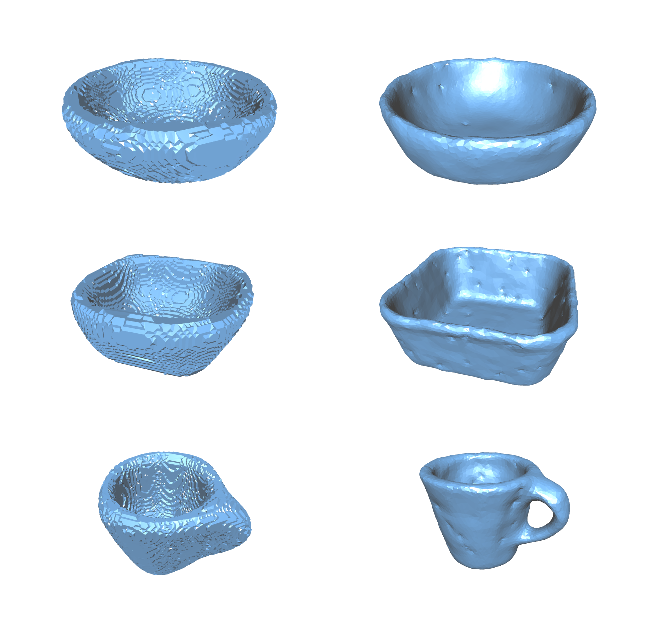
\includegraphics[width=0.95\columnwidth]{comparison.eps}
    \caption{Comparison of reconstructed shapes (left) with the ground truth meshes (right), obtained with our GPAtlasRRT via the Sliding Touch method.}
    \label{fig:shapecomp}
\end{figure}

The setup included three standard personal computers where one was dedicated to the GPAtlasRRT strategy, one acted as the decision-maker and the last was the hardware server. Most of the time is consumed on the computation of the explicit form of the object for collision-avoidance motion planning. Basically, a suggested tactile action could be discarded due to inaccessibility. In such a situation, another touch candidate is requested. Note that, both the GPAtlasRRT strategy and the motion planner are probabilistic, and their combination in some cases led to the planner being trapped in a local-minima.

\begin{figure}
\centering
%\mbox{
  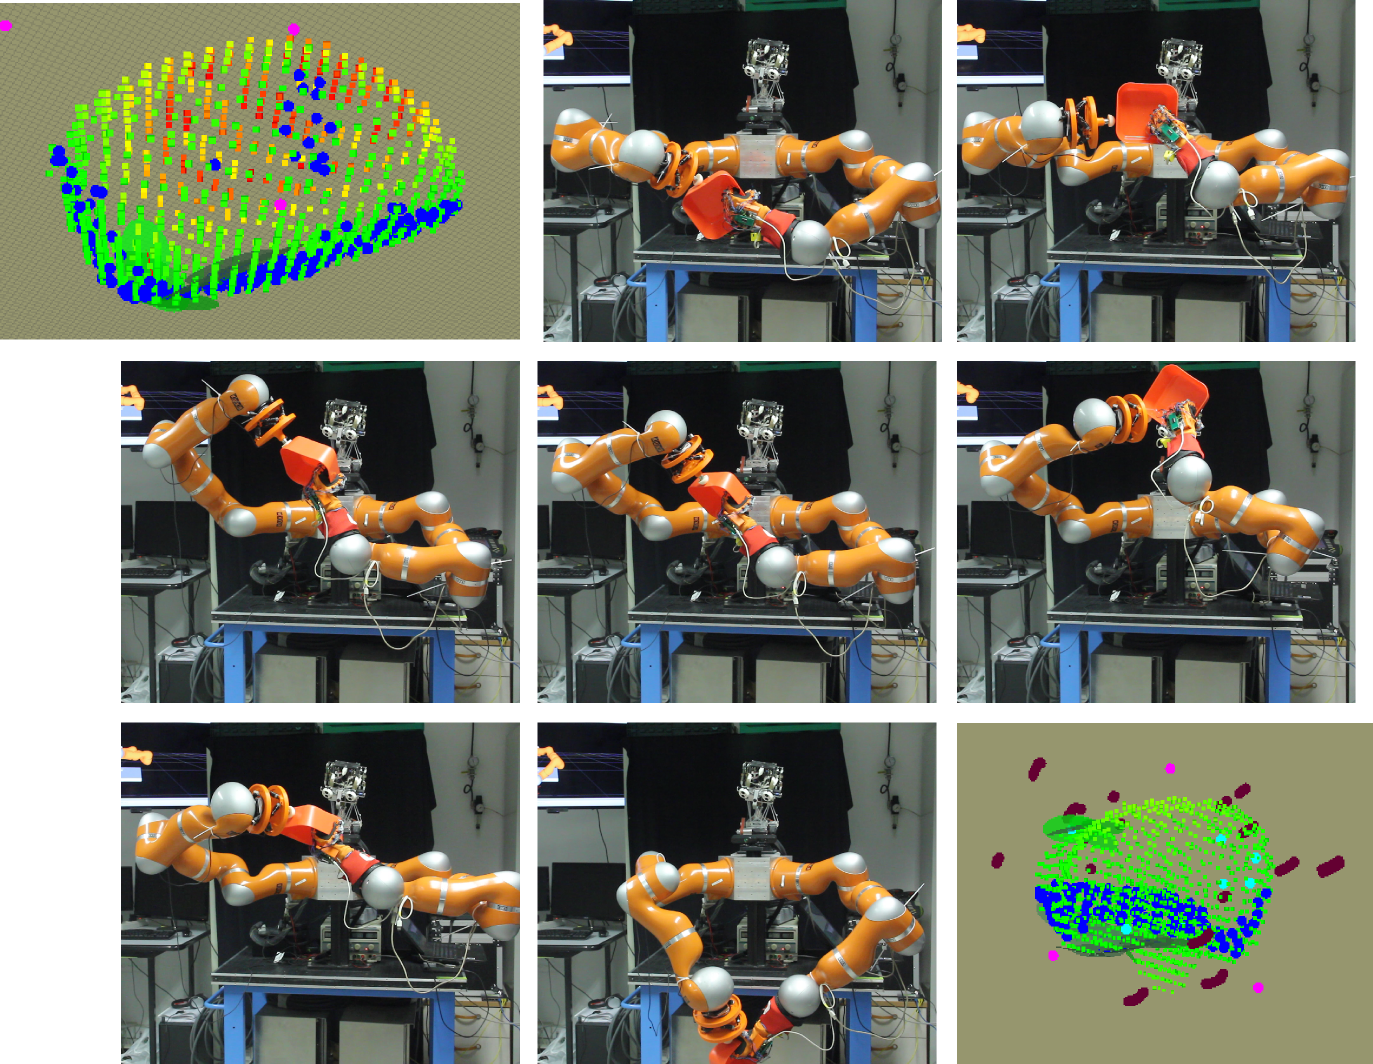
\includegraphics[width=0.9\linewidth]{real_shots.png}
%}
\caption{Our Vito robot performs a tactile exploration action using the proposed GPAtlasRRT strategy. The per-point colour code  is the same as in Fig.~\ref{fig:setup_solution}}
\label{fig:real}
\end{figure}

%%%%%%%%%%%%%%%%%%%%%%%%%%%%%%%%%%%%%%%%%%%%%%%%%%%%%%%%%%%%%%%%%%%%%%%%%%%%%%%%
\section{Conclusions and future work}
\label{sec:conclusions}

We have developed...

As an immediate future research is the study of manifold Gaussian Process as presented by~\citet{Calandra2014Manifold}, so the application of the AtlasRRT as presented by~\citet{Jaillet2013Path} can be applied in a more precise manner.

%%%%%%%%%%%%%%%%%%%%%%%%%%%%%%%%%%%%%%%%%%%%%%%%%%%%%%%%%%%%%%%%%%%%%%%%%%%%%%%%
\begin{acknowledgements}
The authors would like to thank E. Farnioli for the fruitful discussions and initial matlab implementations about Gaussian Processes, as well as to G. Santaera for the support with the sensorized glove.
\end{acknowledgements}

%%%%%%%%%%%%%%%%%%%%%%%%%%%%%%%%%%%%%%%%%%%%%%%%%%%%%%%%%%%%%%%%%%%%%%%%%%%%%%%%
\bibliographystyle{spbasic}
\bibliography{bib/report,bib/marco}

\end{document}
% end of file

%%%%%%%%%%%%%%%%%%%%%%%%%%%%%%%%%%%%%%%%%%%%%%%%%%%%%%%%%%%%%%%%%%%%%%%%%%%%%%%%
%% HELPS
% \begin{equation}
% a^2+b^2=c^2
% \end{equation}
%
% \begin{figure}
% \centering
%   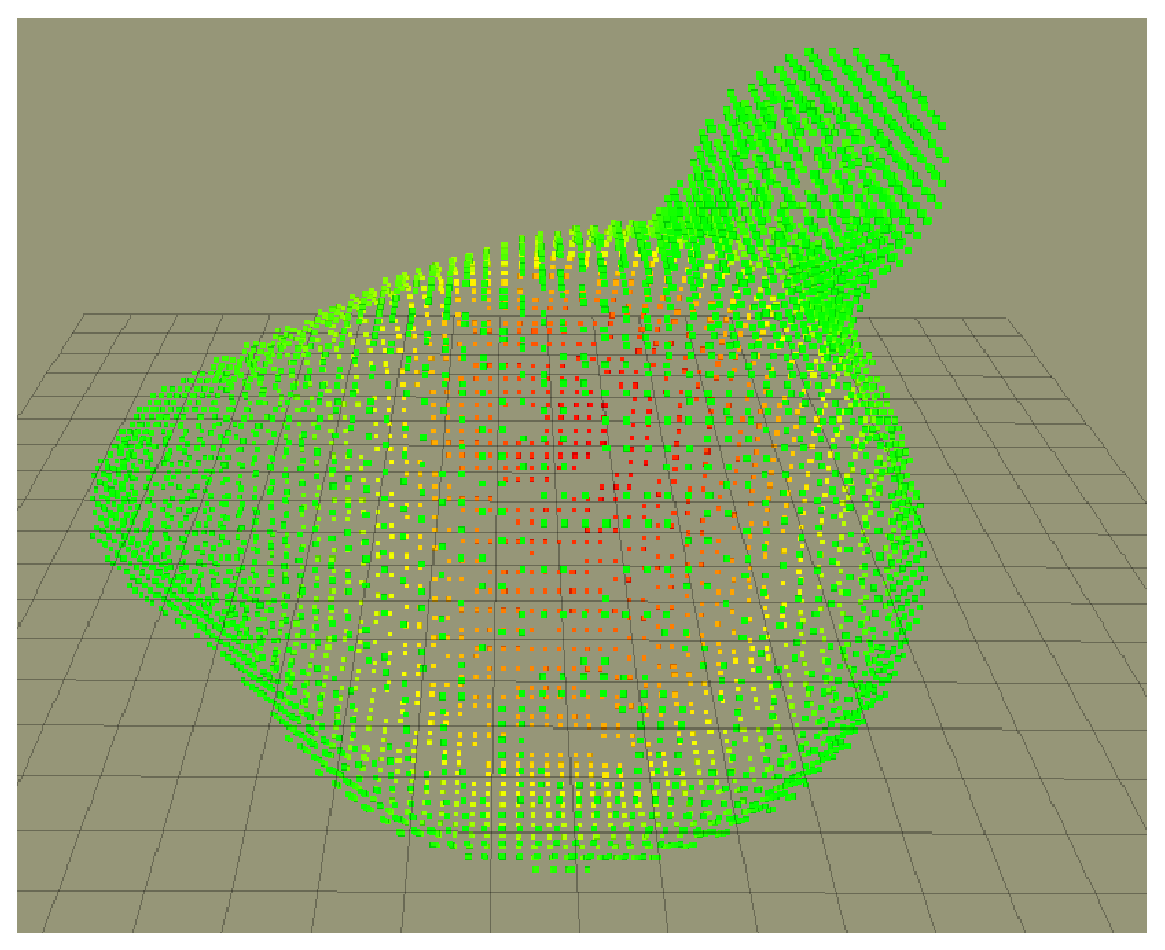
\includegraphics{example.eps}
% \caption{Please write your figure caption here}
% \label{fig:1}
% \end{figure}
%
% \begin{figure*}
% \centering
%   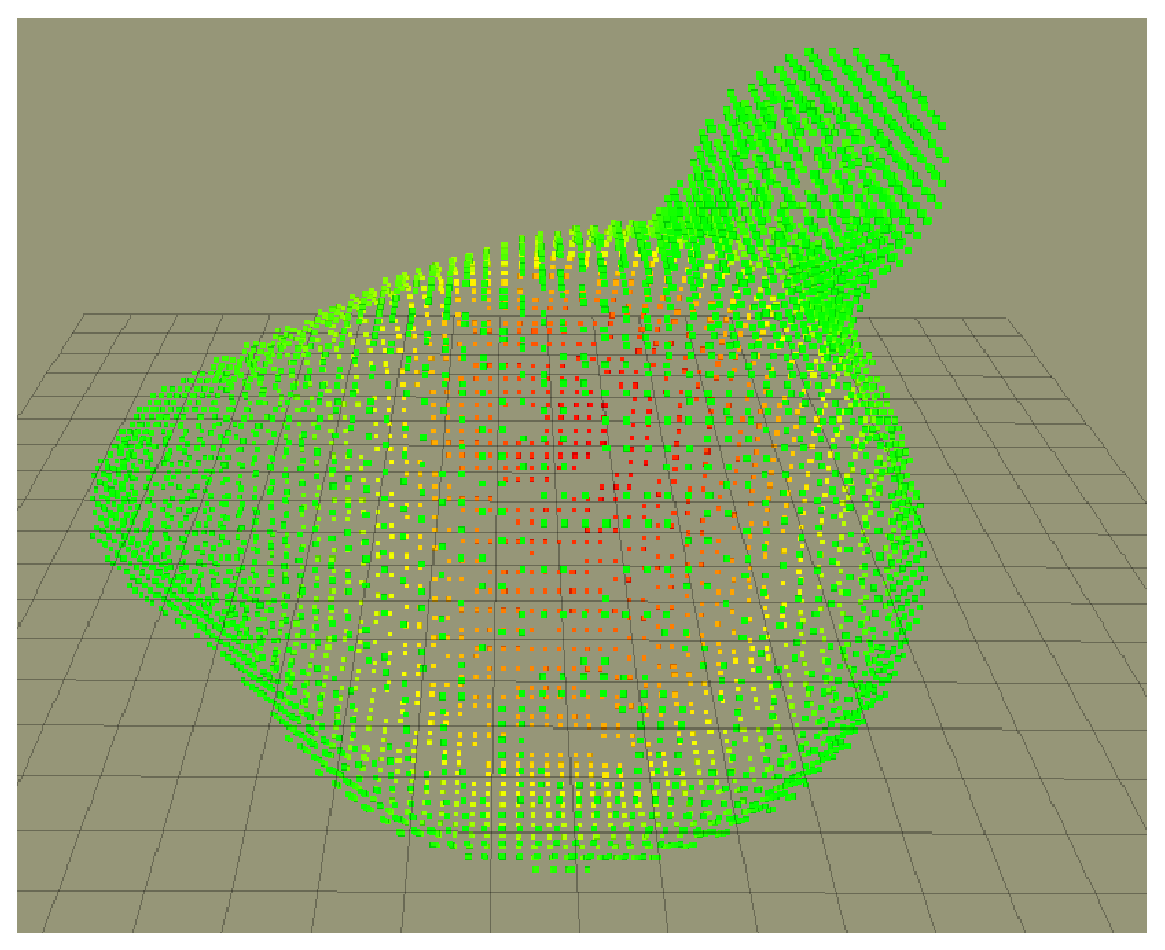
\includegraphics[width=0.75\textwidth]{example.eps}
% \caption{Please write your figure caption here}
% \label{fig:2}
% \end{figure*}
%
% % For tables use
% \begin{table}
% \caption{Please write your table caption here}
% \label{tab:1}
% \begin{tabular}{lll}
% \hline\noalign{\smallskip}
% first & second & third  \\
% \noalign{\smallskip}\hline\noalign{\smallskip}
% number & number & number \\
% number & number & number \\
% \noalign{\smallskip}\hline
% \end{tabular}
% \end{table}
%%%%%%%%%%%%%%%%%%%%%%%%%%%%%%%%%%%%%%%%%%%%%%%%%%%%%%%%%%%%%%%%%%%%%%%%%%%%%%%% 
